\documentclass[12pt,reqno]{amsart}
\usepackage[margin=3cm]{geometry}

\usepackage{amsmath, amssymb, amsfonts, tikz,enumerate, graphicx, textcomp, caption, wrapfig, amsthm, todonotes, verbatim, cleveref, caption, float, mathabx, flafter, url, adjustbox}
\usetikzlibrary{calc, arrows}
\usepackage[procnames]{listings}
\usepackage{color, subfig}
\usepackage[section]{placeins}

\usepackage{color}
\definecolor{purple}{rgb}{0.5,0,1}

\newenvironment{dami}{
  \medskip
\begin{color}{blue}
    \textcolor{purple}{\textbf{Dami:}} 
}{
\end{color}
  \medskip
}


\newenvironment{cat}{
  \medskip
\begin{color}{red}
    \textcolor{red}{\textbf{Catherine:}} 
}{
\end{color}
  \medskip
}

\definecolor{keywords}{RGB}{255,0,90}
\definecolor{comments}{RGB}{0,0,113}
\definecolor{red}{RGB}{160,0,0}
\definecolor{green}{RGB}{0,150,0}
\lstdefinelanguage{Magma}%
  {%
   otherkeywords={:=,+:=,-:=,*:=},%
          % functions
   procnamekeys={function,func,intrinsic,procedure,proc},%
         % Booleans
   morekeywords={true,false},%
          % relations
   morekeywords=[2]{adj,and,cat,cmpeq,cmpne,diff,div,eq,ge,gt,in,is,join,le,lt,%
          meet,mod,ne,notadj,notin,notsubset,or,sdiff,subset,xor},%
          % keywords
   morekeywords=[3]{assigned,break,by,case,catch,continue,declare,default,%
          delete,do,elif,else,end,eval,exists,exit,for,forall,fprintf,if,local,%
          not,print,printf,quit,random,read,readi,repeat,restore,save,select,%
          then,time,to,try,until,vprint,vprintf,vtime,when,where,while},%
          % directives
   morekeywords=[4]{clear,forward,freeze,iload,import,load},%
          % error checks
   morekeywords=[5]{assert,assert2,assert3,error,require,requirege,requirerange},%
          % constructors
   morekeywords=[6]{car,comp,cop,elt,ext,frac,hom,ideal,iso,lideal,loc,map,%
          ncl,pmap,quo,rec,recformat,rep,rideal,sub},%
          % other constructors (semi-reserved)
   morekeywords=[7]{AbelianGroup,AdditiveCode,AffineAlgebra,Algebra,%
          AssociativeAlgebra,Character,CliffordAlgebra,Design,Digraph,%
          ExtensionField,FPAlgebra,FiniteAffinePlane,FiniteProjectivePlane,%
          Graph,Group,GroupAlgebra,IncidenceStructure,LieAlgebra,LinearCode,%
          LinearSpace,MatrixAlgebra,MatrixGroup,MatrixRing,Monoid,%
          MultiDigraph,MultiGraph,NearLinearSpace,Network,PartialMap,%
          PermutationGroup,PolycyclicGroup,QuaternionAlgebra,Semigroup,%
          ZModule},%
          % functions
   morekeywords={[8]function,func,intrinsic,procedure,proc,return},%
      sensitive,%
      morecomment=[l]//,%
      morecomment=[s]{/*}{*/},%
      morecomment=[s]{\{}{\}},%
      morestring=[b]"%
  }[keywords,procnames,comments,strings]%
\lstset{language=Python, 
        basicstyle=\ttfamily\small, 
        keywordstyle=\color{keywords},
        commentstyle=\color{comments},
        stringstyle=\color{red},
        breaklines=true,
        showstringspaces=false,
        identifierstyle=\color{green},
        procnamekeys={def,class}}
%\usepackage[T1]{fontenc}
%\usepackage[urw-garamond]{mathdesign}
\usepackage{tikz-cd}\tikzset{node distance=2cm, auto}
\DeclareMathOperator{\Aut}{Aut}
\DeclareMathOperator{\Hom}{Hom}
\DeclareMathOperator{\Jac}{Jac}
\DeclareMathOperator{\Alt}{Alt}
\DeclareMathOperator{\Sym}{Sym}
\DeclareMathOperator{\Corr}{Corr}
\DeclareMathOperator{\im}{im}
\DeclareMathOperator{\uncurry}{uncurry}
\DeclareMathOperator{\Pic}{Pic}
\DeclareMathOperator{\Div}{Div}
\newcommand{\C}{\mathbb{C}}
\newcommand{\Z}{\mathbb{Z}}
\newcommand{\F}{\mathbb{F}}
\newcommand{\G}{\mathbb{G}}
\newcommand{\Q}{\mathbb{Q}}
\newcommand{\R}{\mathbb{R}}
\newcommand{\n}{\newline}
\newcommand{\mc}{\mathcal}
\newcommand{\te}{\text}
\newcommand{\bb}{\mathbb}
\renewcommand{\P}{\mathbb{P}}
\newcommand{\BBF}{\overline{\F_p}}
\newcommand\mapsfrom{\mathrel{\reflectbox{\ensuremath{\mapsto}}}}
\definecolor{codegray}{gray}{0.9}
\newcommand{\code}[1]{\colorbox{codegray}{\texttt{#1}}}
\newtheorem{theorem}{Theorem}
\newtheorem*{thm*}{Theorem}
\newtheorem*{proposition}{Proposition}
\newtheorem{lemma}[theorem]{Lemma}
\newtheorem*{lemma*}{Lemma}
\newtheorem*{qlemma*}{``Lemma"}
\newtheorem{cor}[theorem]{Corollary}
\newtheorem*{conjecture*}{Conjecture}
\newtheorem{postulate}[theorem]{Postulate}
\newtheorem*{question}{Question}
\theoremstyle{definition}
\newtheorem{defn}{Definition}
\newtheorem{example}[theorem]{Example}
\theoremstyle{remark}
\newtheorem*{remark}{Remark}
\newtheorem*{answer}{Answer}
\newtheorem*{notation}{Notation}
\newtheorem*{note}{Note}
\newcommand{\sss}{\ss$\text{ }$}
\newcommand{\ti}{\todo[inline]}
\newcommand{\DD}{\Delta\kern -8.3pt {\diamond} \kern -4.5pt \cdot \:}
\newenvironment{myproof}[1][``\proofname '']{%
  \proof[ #1]%
}{\endproof}


\title[Automorphisms of Abelian Varieties and Principal Polarizations]{Automorphisms of Abelian Varieties \\ and Principal Polarizations}
\author{Dami Lee and Catherine Ray}

\begin{document}

  
\maketitle

\begin{abstract} Abelian varieties with several principal polarizations are incredibly rare. The still unsolved Narasimhan-Nori conjecture asks for a closed formula for the number of non-isomorphic principal polarizations of any given abelian variety. We give lower bounds on the number of principal polarizations on any given abelian variety by introducing a new computer program.
We show, for example, that the Jacobian of Schoen's I-WP minimal surface has at least 9 non-isomorphic principal polarizations. We also explore the Jacobians of Klein's quartic, Fermat's quartic, Bring's curve, the modular curve $X_0(63)$, and more.   
\end{abstract}

\section{Introduction}

Our paper introduces a new computer program to find multiple non-isomorphic principal polarizations on abelian varieties in characteristic 0, the code for which is publically available. In general, abelian varieties with several principal polarizations are incredibly rare. In fact, abelian varieties with no principal polarizations are, in some sense, dense on the moduli stack of abelian varieties. %(considered in terms of their big Period matrix).

The fact that an abelian variety admits only a finite number of isomorphism classes of principal polarizations was established by Narasimhan-Nori. In \cite{nn}, they pose the problem of finding a closed formula for the number of principal polarizations of any given abelian variety over any field, which is still unsolved. 

In this paper, we introduce an entirely different technique to find different principal polarizations on Jacobians, exposited in Section ~\ref{sec:find}, which treats both simple and non-simple cases in characteristic 0. We use this to give lower bounds on the number of non-isomorphic principal polarizations. For example, we have the following result. 

\begin{theorem} \label{IWP} Let $\pi(X)$ denote the number of non-isomorphic principal polarizations on any given variety $X$. Let I-WP denote Schoen's I-WP surface, and $\Jac(\text{I-WP})$ its Jacobian variety, then $$\pi(\Jac(\text{I-WP})) \geq 9.$$\end{theorem}

This is a charming result, especially since the variety $\Jac(\text{I-WP})$ itself factors into a product of 4 elliptic curves\footnote{This is because $\text{End}(\Jac(\text{I-WP})) \simeq M_4(K)$, where $K$ is imaginary quadratic. Thus, $\Jac(\text{I-WP})$ is the product of elliptic curves with CM by $K$.}, so the remaining principal polarizations must come from interesting new cycles in the product of these elliptic curves. Other such surprising results found by applying our technique are shown in Table ~\ref{table:tablelabel}, Section ~\ref{sec:examples}.

Our method works as follows. For curves that are cyclic covers over $\C\bb{P}^1$, we can compute exact period matrices, exposited in Section ~\ref{sec:cyclicperiod}; otherwise, we compute the period matrices numerically. Given any period matrix, we introduce new code to compute many principal polarizations on the corresponding abelian variety.  Then, we implement a modification of the psuedocode of Bruin-Jeroen-Sijsling \cite{numerical} to compute, for each found principal polarization, the automorphism group of the given Jacobian which fixes that polarization. If the automorphism groups are different, then the principal polarizations are non-isomorphic. This gives us a lower bound on the number of different principal polarizations for a given Jacobian. The fact that numerical computations with period matrices, which we use for surfaces which are not cyclically branched covers of $\C\P^1,$ give rigorous results relies on the brilliant work of Costa-Mascot-Sijsling-Voight (\cite{rigor} Prop 6.1.1), which we discuss in Section ~\ref{sec:cert}.

We demonstrate the power of our method with a variety of different period matrices. We exposit some low dimensional geometry which allows us to compute exact period matrices of cyclically branched covers of $\C\P^1.$ We also work with period matrices of modular curves, as codified by Mascot in a slight modification of \cite{n} toward computing Galois representations. These modular curves are not cyclically branched covers over $\C\P^1,$ and thus give us a completely disjoint collection of curves to which we apply our methods. Assuming that our program finds \textit{all} principal polarizations of any given abelian variety, we give a new proof of the automorphism group of $X_0(63)$, which was the only remaining unresolved automorphism group of a compact modular curve until 1990 \cite{elkies}.  


\section*{Acknowledgements} 
Lee would like to thank Matthias Weber for his guidance at the beginning of this project. Ray would like to thank \texttt{Magma} and \texttt{Sage} contributors John Voight, Edgar Costa, Nicolas Mascot, and above all Jeroen Sijsling, who generously offered incredibly detailed and consistent help in computing the automorphism groups of Jacobians.  This material is based upon work supported by the National Science Foundation under Grant No. DMS-1440140 while Lee was in residence at the Mathematical Sciences Research Institute in Berkeley, California, during the Fall 2019 semester. Ray is partially supported the National Science Foundation GRFP under Grant Number DGE 1842165.

\section{Summary of Prior Work}

We summarize what is known about abelian varieties with several principal polarizations. The previous work toward the Narasimhan-Nori conjecture can be divided into the simple and non-simple cases, in which we can further divide into the characteristic 0 or characteristic $p$ cases. An abelian variety is simple if it is not isogenous to a product of abelian varieties of lower dimension. 

We review first prior work toward understanding the case of \textit{simple} varieties in characteristic 0. In \cite{several} Theorem 1.5, Lange establishes for simple varieties that the order of $\Aut(A)$ with certain restriction conditions and equivalence relations is equal to the number of principal polarizations on $A$ up to isomorphism, $\pi(A)$. One could in principal compute the size of this specially carved out version of $\Aut(A)$ by hand using Lange's theorem, however, it is computationally infeasible. This is incredible, it gives us a set equivalence between a slighly carved automorphism group of a variety, and its set of principal polarizations.

%\begin{remark} His bijection between sets is induced by considering an element in the Neron-Severi group of $A$, and representing such elements as endomorphisms of $A$ preserved under the Rosati involution with respect to a chosen polarization. Since this bijection is induced by a principal polarization, one must know that one exists to implement this theorem. \end{remark}


\begin{remark} In Theorem 3.1 \cite{several}, Lange further establishes bounds on $\pi(A)$ in terms of the class group of $End_{\Q}(A)$, if $End_{\Q}(A)$ is a \textit{totally real} number field $K$ (and thus the variety $A$ is simple). \end{remark}  

More recently, Lange treated the non-simple case of products of elliptic curves without complex multiplication in Theorem 3.5 \cite{newlange}. He did so by giving an interpretation of the number of principal polarizations in terms of class numbers of definite Hermitian forms.

%\begin{remark} The main idea of the proof of 3.5 is that the canonical principal polarization of X induces a bijection between P(X) and the set of equivalence classes of symmetric automorphisms of X. Via the analytic representation of X and a suitable choice of bases this set can be considered as a set of equivalence classes of Hermitian forms. \end{remark}

All other previous works known to the authors on finding multiple principal polarizations on abelian varieties have been done by finding two non-isomorphic curves with the same (unpolarized) Jacobian. Therefore, their associated canonical polarizations must be different by the Torelli theorem. Otherwise, the curves would be isomorphic. All papers that we know of using this technique do so only in characteristic $p$. 

\begin{remark} There is only a canonical principal polarization on $A$ if a curve $C$ is specified so that $A = \Jac(C).$ If $C$ is not specified, there is no canonical choice -- knowing that $A$ is in the image of the functor $\Jac$ is not enough. Thus, there can be several ``canonical" principal polarizations on one Jacobian, its canonicality only refers to the fact that it comes from a curve. \end{remark}

The papers using this non-isomorphic curve technique discuss the case of \textit{non-simple} Jacobians of curves of genus two \cite{iko} and three [Brock, \textit{Superspecial curves of genera two and three}], though we were unable to find a copy of the latter. 

This technique is again used by E. Howe \cite{howe1} and \cite{howe2} which gives examples of non-isomorphic genus two curves with the same \textit{simple} Jacobian. He finds such examples in characteristic $p$ by playing with isogeny classes of abelian varieties which correspond to special Weil numbers, an application of the Honda-Tate method. This summarizes all previous work known to the authors.


\section{Background}
\label{sec: dthesis}
In \cite{dthesis}, Lee classifies curves with cone metrics that are realizable as a quotient of a triply periodic surface embedded in $\R^3.$ By triply periodic, we mean that the surface is invariant under a rank-three lattice $\Lambda \subset \R^3.$ Specifically, they consider curves that are cyclically branched over $\mathbb{C}\mathbb{P}^1,$ hence we will devote this section to providing the background. This section is a summary of Chapter 3 \cite{dthesis}. 

\subsection{Cone Metrics}
First, we discuss the topological construction of cyclic covers over $\mathbb{C}\mathbb{P}^1.$ This will naturally yield cone metrics on the curves.

\subsubsection*{Construction of cyclic covers over $\mathbb{C}\mathbb{P}^1$}
\begin{defn} We say that a curve $C$ is a $d$-fold cyclic cover over $\mathbb{C}\mathbb{P}^1$ if $C / (\Z/ d \Z) = \mathbb{C}\mathbb{P}^1.$ \end{defn}

We construct such curves with the given data: let $p_i, \ldots , p_n \in \mathbb{C}\mathbb{P}^1$ be $n$ distinct points. Let $Y := \mathbb{C}\mathbb{P}^1 \backslash \{p_1, \ldots, p_n\}$ and let $\gamma_i$ be a branch cut from $p_i$ to some $q \in Y$ so that $\gamma_i$ are mutually disjoint. For each $i,$ assign $d_i \in \{1, \ldots, d - 1\}$ and call it the \textbf{branching index at} $p_i.$ Let $d$ be the degree of the covering map and use $j$ to label $Y_1, \ldots , Y_d.$ For each $i$ and $j,$ we identify the ``left side'' of $\gamma_i$ of $Y_j$ to the ``right side'' of $\gamma_i$ of $Y_{j + d_i \pmod d}.$ We denote such a covering $C$ by a $d$-tuple $d (d_1, \ldots , d_n).$


\begin{remark} A covering $d (d_1, \ldots , d_n)$ is uniquely defined up to homeomorphism. That is, the construction only depends on $d_i$ and is independent of $p_i,$ $\gamma_i,$ and $q.$ We will assume that $\sum\limits_{i=1}^n d_i \equiv 0 \pmod d$ and also $\gcd (d_1, \ldots, d_n) = 1.$ The former guarantees that the covering is closed and the latter guarantees that the covering is connected. In fact, both are sufficient and necessary conditions. Then one can compute the genus of the curve by Riemann-Hurwitz formula and $g(C) = \frac{d (n-2)}{2} + 1 - \frac{1}{2} \sum\limits_{i=1}^n \gcd(d,d_i).$ 
\end{remark}

\subsubsection*{Branching indices on Octa-4}
As a running example, we will look at the curve from \cite{dami}. It is there called Octa-4 due to the formation of the triply periodic surface. It is also shown that the underlying curve is conformally equivalent to Fermat's quartic. The underlying genus three curve $C$ (Figure~\ref{fig:125}) is invariant under an order-eight rotational symmetry. The curve is an eightfold cyclic cover over $\mathbb{C}\mathbb{P}^1$ denoted as $8 (1, 2, 5).$

\begin{figure}[htbp] 
   \centering
   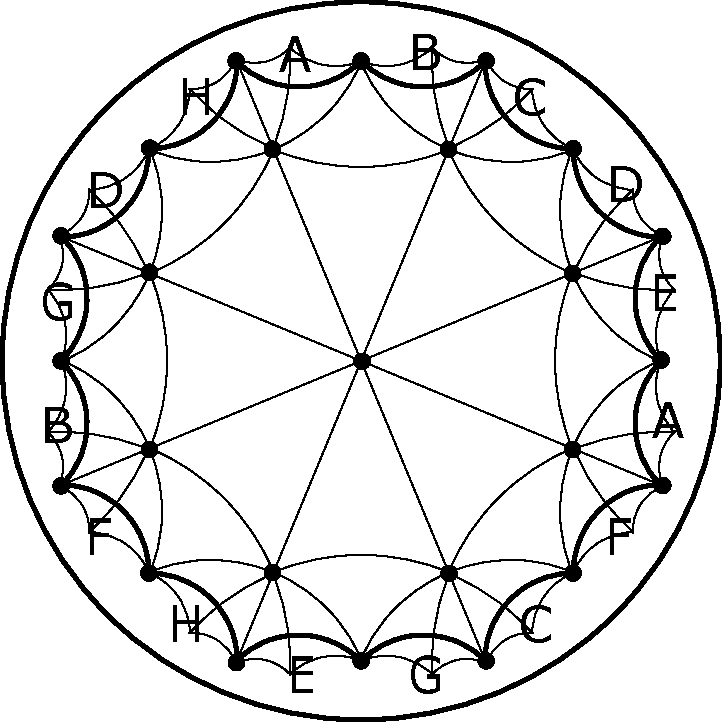
\includegraphics[width=2in]{figures/125_base.pdf} 
  \caption{Hyperbolic tessellation on $8(1, 2, 5).$ Reprinted from \cite{dami}.}
  \label{fig:125}
\end{figure}

%The euclidean triangles on the fundamental piece of $\Pi$ have a one-to-one correspondence to the hyperbolic triangles.

For each $i,$ there are $\gcd(d, d_i)$ preimages $\widetilde{p_i}$ of $p_i$ on $C.$ Hence, each $\widetilde{p_i}$ is a non-trivial cone point. To pin down a holomorphic 1-form on $C,$ we find cone metrics on $\mathbb{C}\mathbb{P}^1$ and pull-back to its covering. We say that a cone metric on $\mathbb{C}\mathbb{P}^1$ is \textbf{admissible} if its pullback yields a flat structure on $C.$ The following proposition is a version of Gauss-Bonnet theorem.

\begin{proposition} Given a compact Riemann surface of genus $g$ with a cone metric, let $p_1, \ldots, p_n$ be distinguished points with respective cone angles $\theta_i.$ Then $\sum\limits_{i=1}^n \theta_i = 2 \pi (2 g - 2 + n).$
\end{proposition}

Specifically, the sum of cone angles on a genus zero curve is $2 \pi (n - 2).$ Given branching indices such that $\sum\limits_{i=1}^n d_i = d (n - 2),$ we get a cone metric on the Riemann sphere with cone angles $\frac{2 \pi d_i}{d}$ at each $p_i.$ For example, by putting a cone metric on the quotient sphere where the cone angles are $\frac{1 \pi}{4}, \frac{2 \pi}{4},$ and $\frac{5 \pi}{4}$ as in Figure~\ref{fig:125_flat}, one can see that the identification of edges are by translations. In other words, this gives rise to a translation structure on the eightfold cover of the sphere. Moreover, we obtain a holomorphic 1-form with one order-4 zero.

\begin{figure}[htbp]
   \centering
   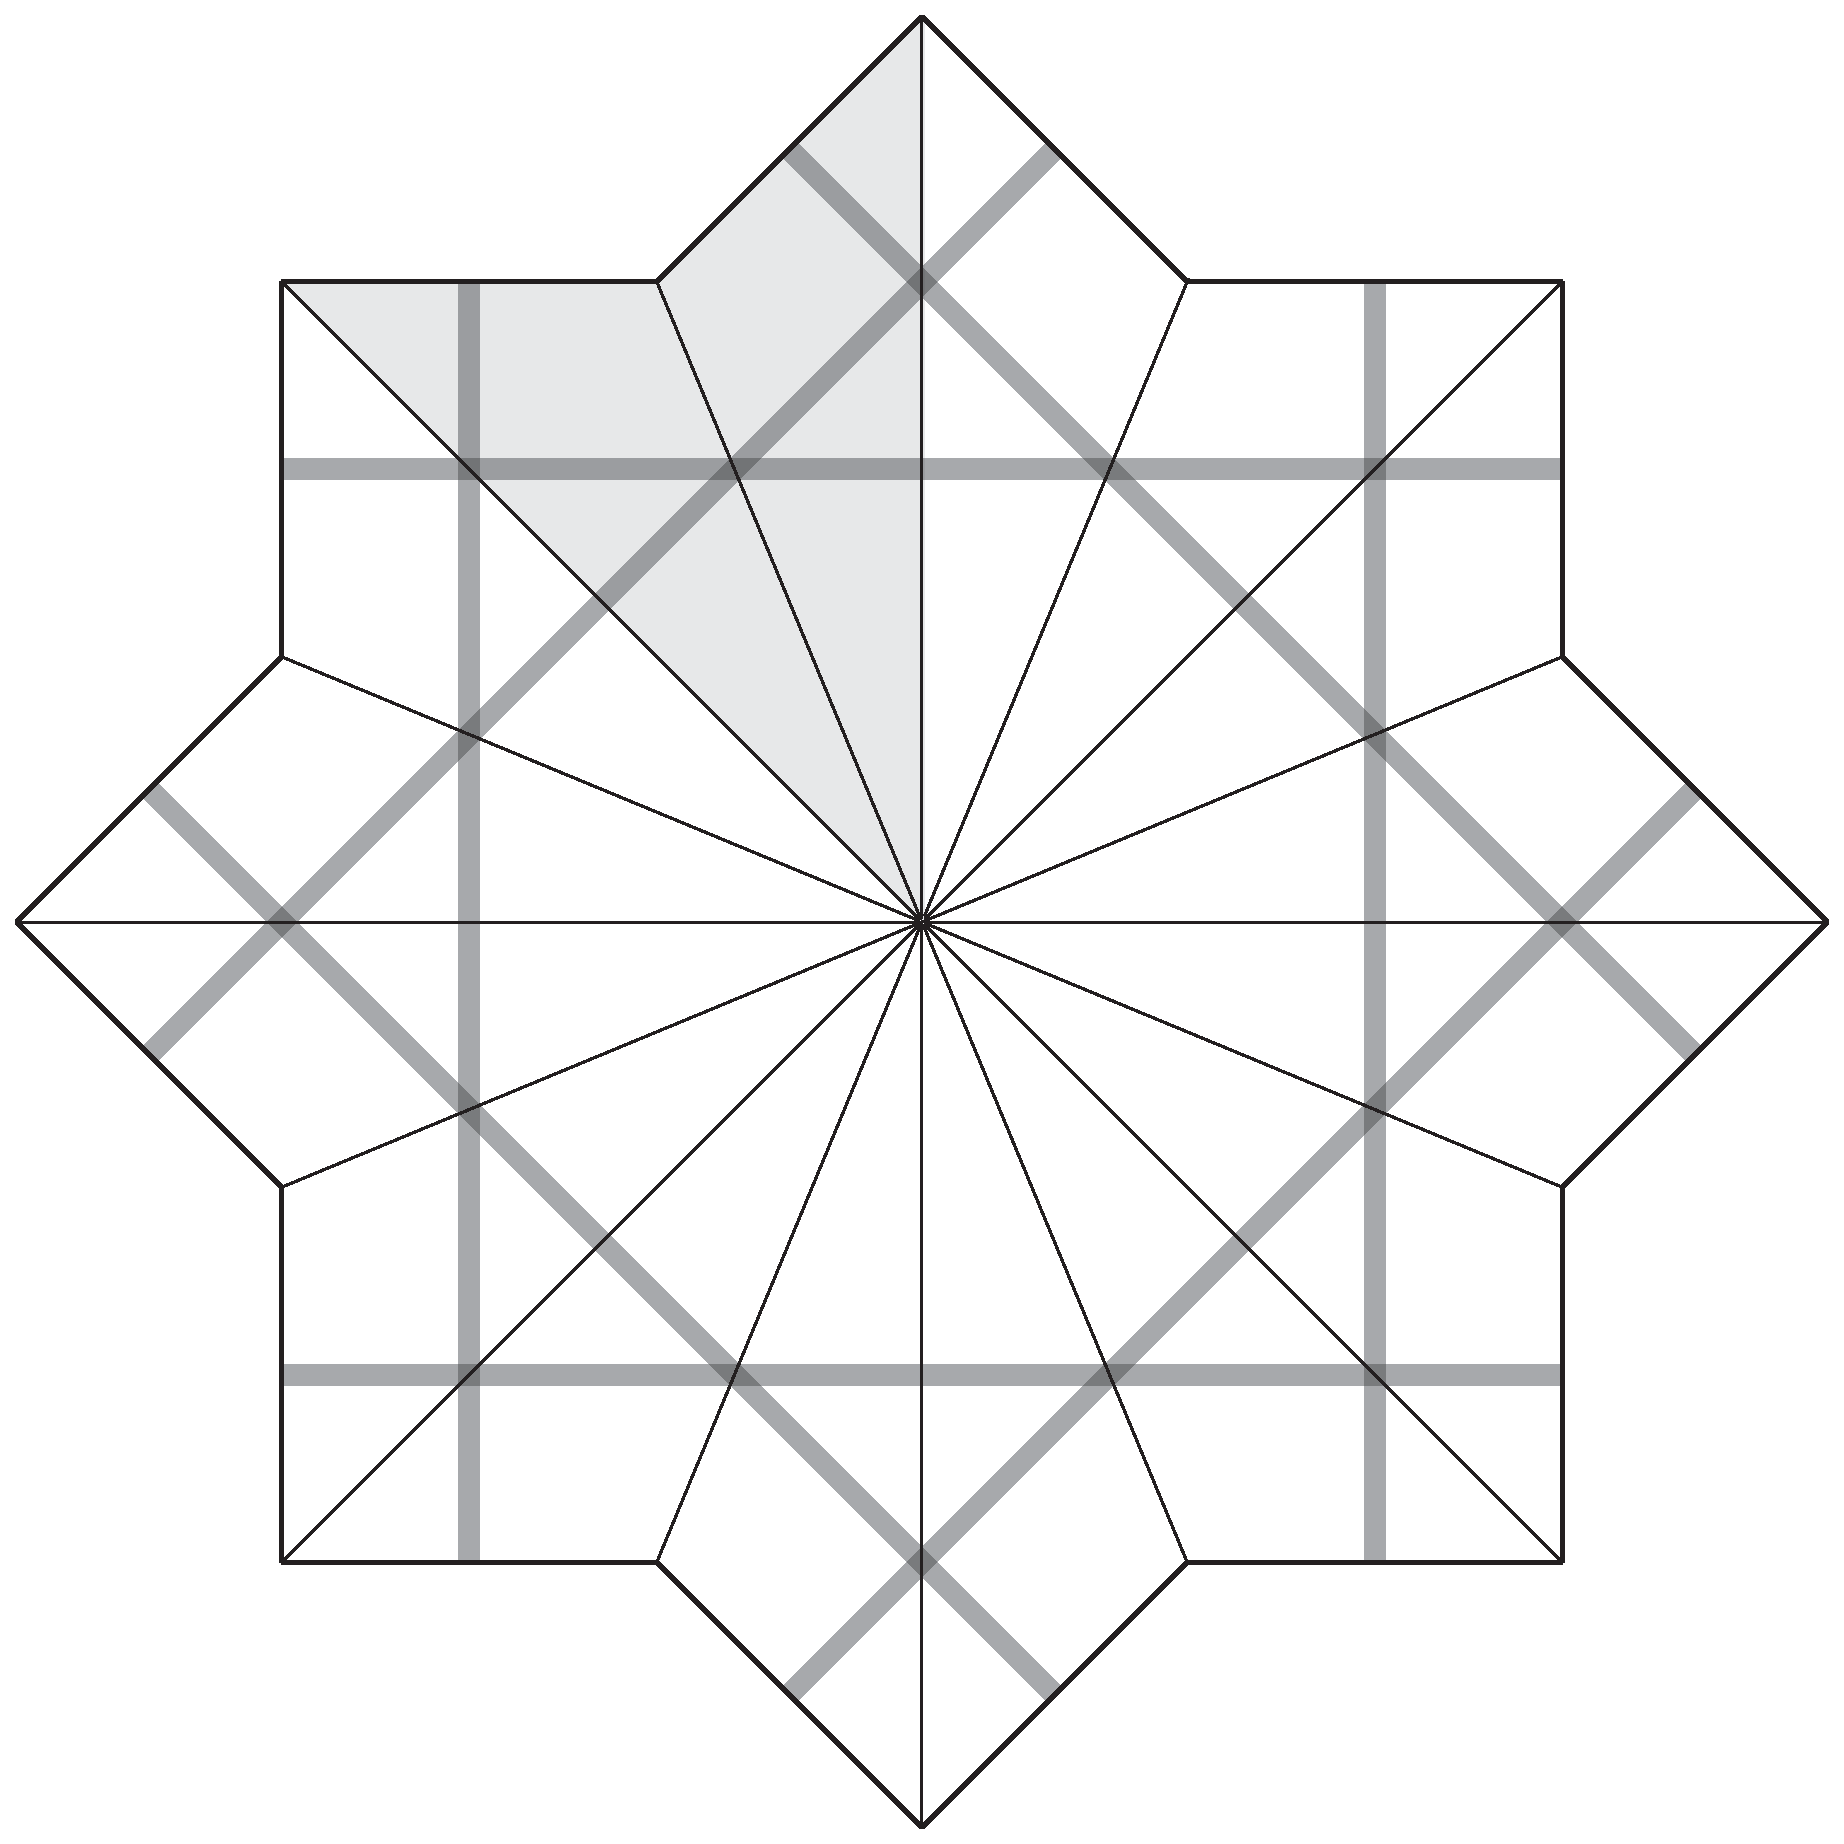
\includegraphics[width=2.5in]{figures/125_flat.pdf} 
  \caption{A flat structure $\omega_1$ on $8(1, 2, 5)$ with one marked zero. Modified from \cite{dami}}
  \label{fig:125_flat}
\end{figure}

Our goal is to find other admissible cone metrics on the sphere that yield different translation structures (linearly independent 1-forms) on the same curve. We claim that the cone metric given by cone angles $\frac{2 \pi a_i}{d}$ where $a_i \equiv d_i \pmod d$ for all $i$ is admissible (Theorem 3.4, \cite{dthesis}). An easier way of finding admissible cone metrics is given by the following notion of multipliers.

\begin{defn} Given branching indices $d (d_1, \ldots , d_n),$ we say $a \in \{1, \ldots, d - 1\}$ is a \textbf{multiplier} if the cone metric given by cone angles $\frac{2 \pi}{d} (a \cdot d_1 \pmod d, \ldots , a \cdot d_n \pmod d)$ is admissible. 
\end{defn}

Theorem 3.5, \cite{dthesis} proves that for $n = 3,$ there are exactly $g$ multipliers. In other words, one achieves a basis of holomorphic 1-forms via multipliers. We denote the multipliers by $a_i,$ hence the admissible cone angles are given by $$\frac{2\pi}{d}(a_1 d_1, a_1 d_2, a_1 d_3), \ldots , \frac{2\pi}{d}(a_g d_1, a_g d_2, a_g d_3).$$ 

\subsubsection*{Admissible cone metrics on Octa-4} Given branching indices $8 (1, 2, 5),$ multipliers 1, 2, and 5 give rise to cone metrics with cone angles $\frac{2 \pi}{8}(1, 2, 5),$ $\frac{2 \pi}{8}(2, 4, 2),$ and $\frac{2 \pi}{8}(5, 2, 1),$ respectively. These cone metrics yield a basis of holomorphic 1-forms with the following divisors: $$(\omega_1) = 4 \widetilde{p_3}, \qquad (\omega_2) = \widetilde{p_1} + \widetilde{p_2}_1 + \widetilde{p_2}_2 + \widetilde{p_3}, \qquad (\omega_3) = 4 \widetilde{p_1}.$$

Figure~\ref{fig:flat_rs2} represents $\omega_2$ given by cone angles $\frac{2 \pi}{8}(2, 4, 2).$ The four simple zeros are marked on the figure.

\begin{figure}[htbp]
   \centering
   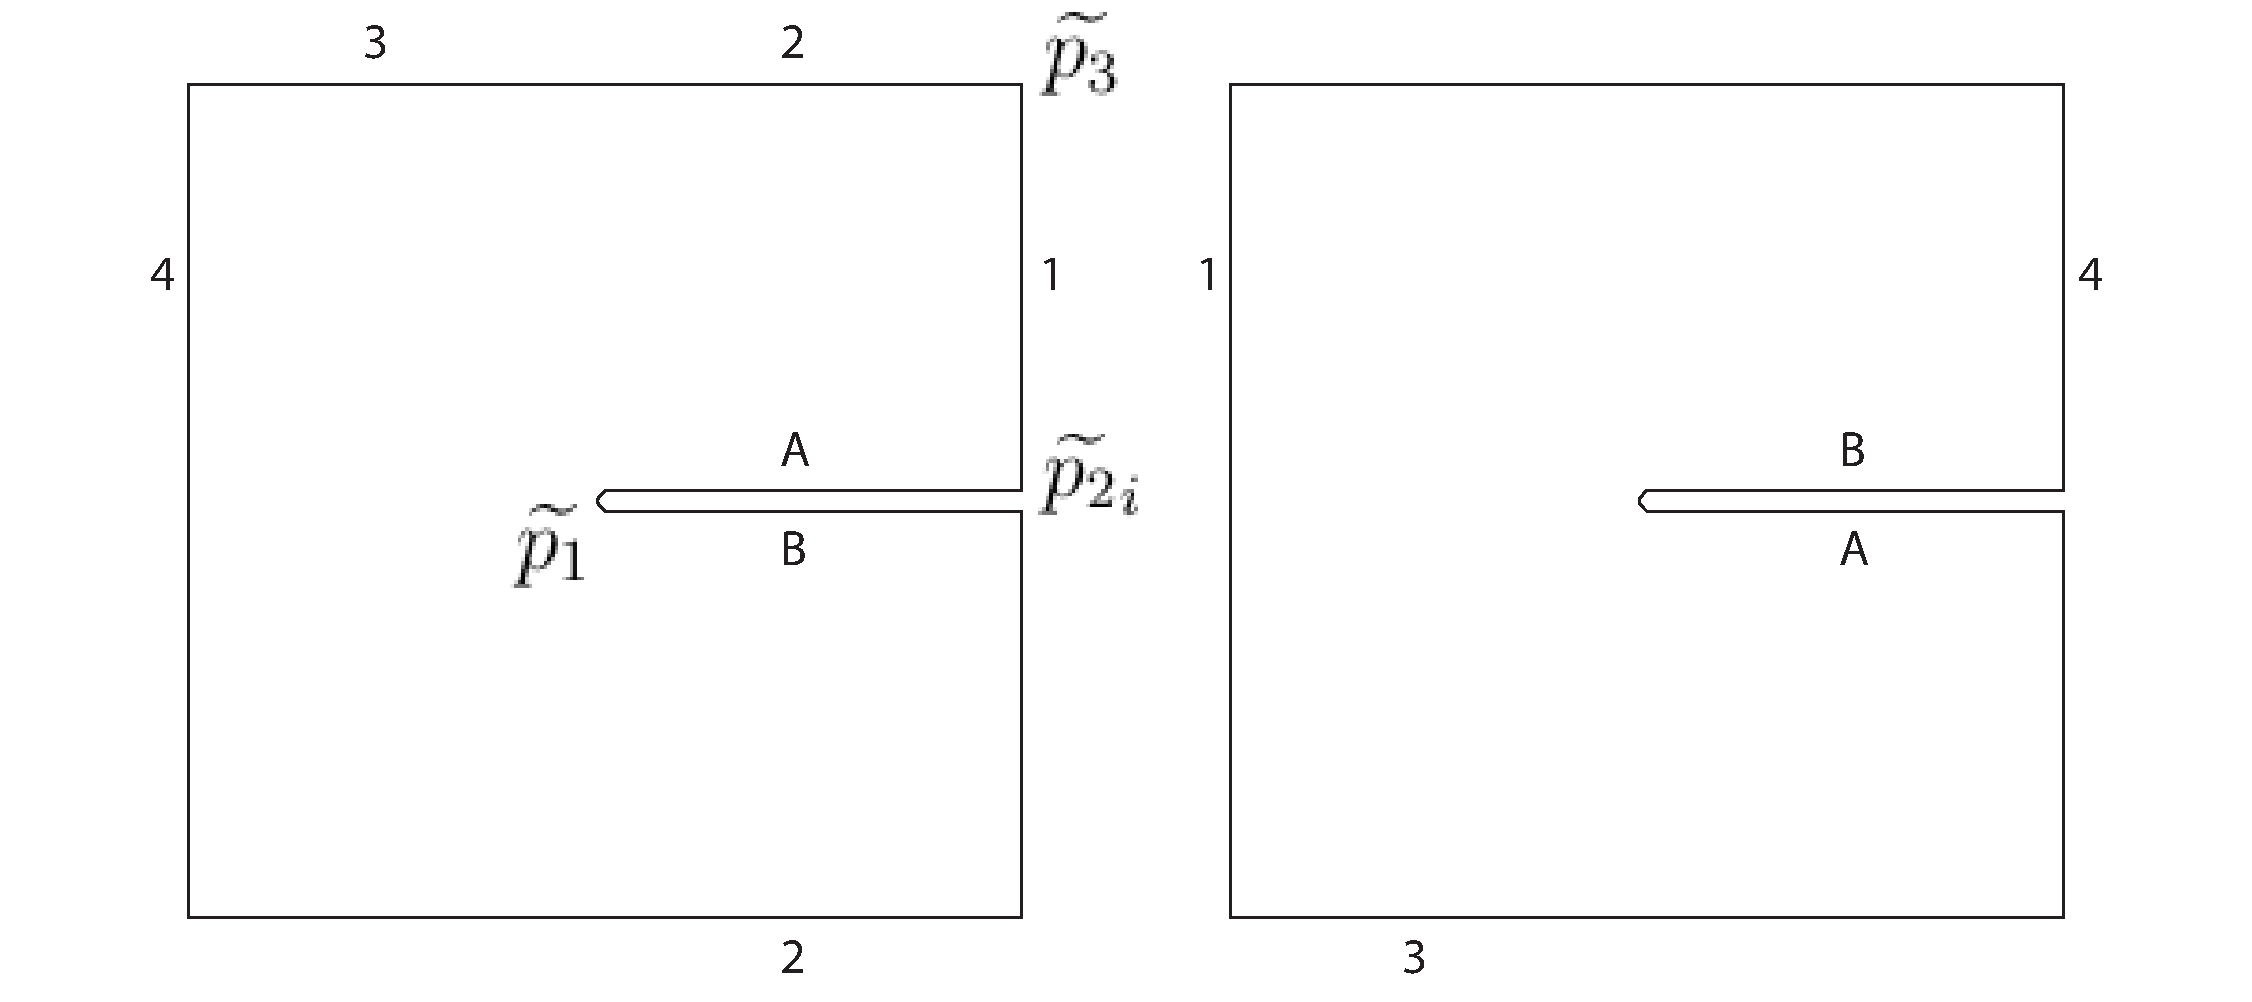
\includegraphics[width=4in]{figures/flat_rs2.pdf} 
  \caption{A flat structure $\omega_2$ on $8(1, 2, 5)$ with four simple zeros. Modified from \cite{dthesis}}
  \label{fig:flat_rs2}
\end{figure}

\begin{remark} Note that the multipliers preserve the labeling of edges in both Figure~\ref{fig:125_flat} and Figure~\ref{fig:flat_rs2}: 1,2,3,4,5,6,2,8,4,7,6,1,8,3,7,5.
\end{remark}

\begin{remark} Note that 3, 6, and 7 are not multipliers as their corresponding forms do not yield canonical divisors. On the other hand, 4 is not a multiplier as the cone metric derived from cone angles $\frac{2 \pi}{8} (4, 0, 4)$ is not admissible. This induces a meromorphic form whose divisor is $3 \widetilde{p_1} - \widetilde{p_2}_1 - \widetilde{p_2}_2 + 3 \widetilde{p_3}.$ \end{remark}

\begin{remark} The geometric representation of $\omega_3$ can also be achieved by reflecting $\frac{\pi}{8}(5, 2, 1)$ triangles. However, we omit the corresponding figure. \end{remark}



\subsection{Computing the Period Matrix on Cyclic Covers}
\label{sec:cyclicperiod}
In this section, we use the flat structure of a surface to compute the period matrix of a given curve. We will look at the simplest case where $n = 3$ and $d_1 = 1.$ Then, since $\sum d_i = d,$ a cone metric with cone angles $\frac{2 \pi}{d}(d_1, d_2, d_3)$ is admissible. $Y$ is topologically equivalent to a doubled triangle with angles $\frac{2 \pi}{d}(d_1, d_2, d_3)$ so we construct $C$ with $d$ copies of $Y,$ which yields a flat structure on $C.$  We will follow the underlying surface of Octa-4 as our leading example.


Figure~\ref{fig:125_flat} shows the flat structures on the underlying surface of Octa-4 \cite{dami}. The identification of edges are via parallel translations, which verifies that the cone metric is admissible. Parallel translations yield closed cycles on the surface from which we get a homology basis with the following intersection matrix

$$\textrm{int}_1 = \begin{pmatrix} 0 & 1 & 1 & 0 & 0 & 0 \\
 -1 & 0 & 1 & 1 & 0 & 0 \\
 -1 & -1 & 0 & 1 & 1 & 0 \\
 0 & -1 & -1 & 0 & 1 & 1 \\
 0 & 0 & -1 & -1 & 0 & 1 \\
 0 & 0 & 0 & -1 & -1 & 0 \end{pmatrix}.$$

Then the period matrix is computed as follows: 
$$\Pi_1 = \left(
\begin{array}{cccccc}
 1 & e^{\frac{\pi i}{4}} & i & e^{\frac{3 \pi i}{4}} & -1 & e^{-\frac{3 \pi i}{4}} \\
 1 & i & -1 & -i & 1 & i \\
 1 & e^{-\frac{3 \pi i}{4}} & i & e^{-\frac{\pi i}{4}} & -1 & e^{\frac{\pi i}{4}} 
\end{array}
\right).$$


In general, from cyclicity we get 

$$\Pi = \left(
\begin{array}{ccccc}
 1 & e^{\frac{2 \alpha_1 \pi i}{d}} & e^{\frac{4 \alpha_1 \pi i}{d}} & \cdots & e^{\frac{2 (2 g - 1) \alpha_1 \pi i}{d}} \\
 1 & e^{\frac{2 \alpha_2 \pi i}{d}} & e^{\frac{4 \alpha_2 \pi i}{d}} & \cdots & e^{\frac{2 (2 g - 1) \alpha_2 \pi i}{d}} \\
 \vdots\\
 1 & e^{\frac{2 \alpha_g \pi i}{d}} & e^{\frac{4 \alpha_g \pi i}{d}} & \cdots & e^{\frac{2 (2 g - 1) \alpha_g \pi i}{d}} \\
\end{array}
\right)$$
where $\alpha_i$ are the multipliers.




\begin{remark} In \cite{dthesis}, Lee computes the period matrix by choosing a different homology basis. In \cite{dami}, Lee shows that the 8(1,2,5) covering has a geometric realization as a quotient of a triply periodic polyhedral surface where the hyperbolic structure of the underlying curve is induced from the polyhedral cone metric. A triply periodic polyhedral surface is a polyhedral surface that is invariant under a rank-three lattice in $\R^3.$ Figure~\ref{fig:funda} is the genus-three quotient of the polyhedral surface via its lattice of translations. 

\begin{figure}[htbp]
   \centering
   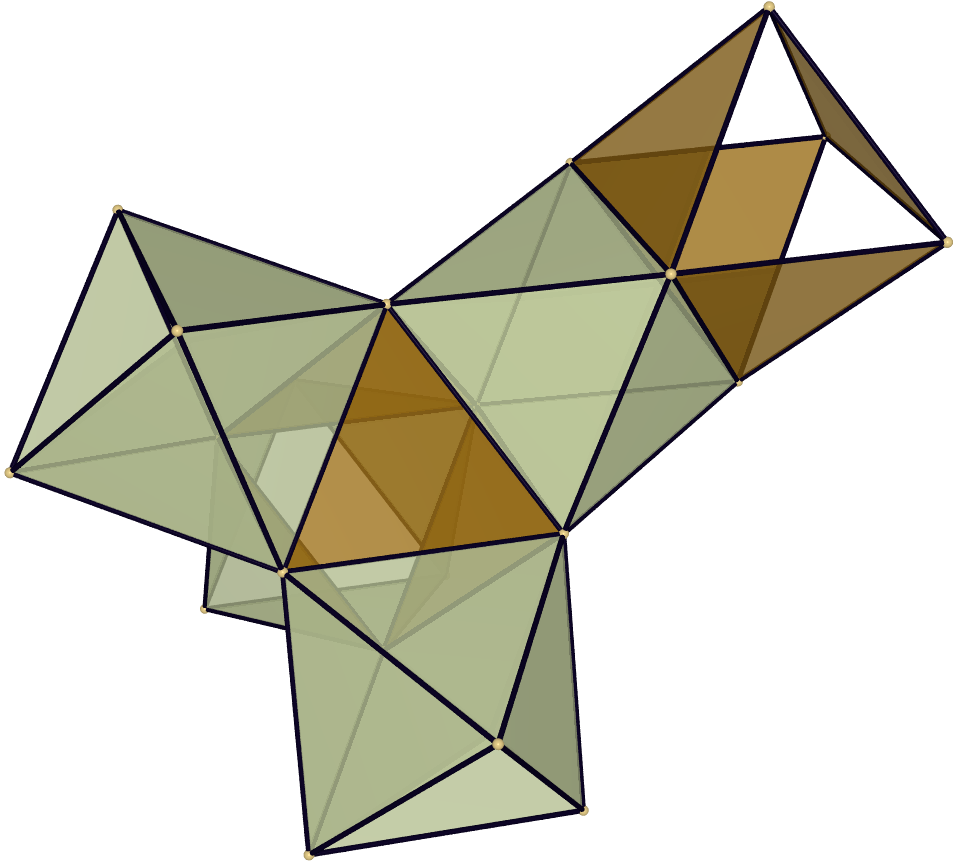
\includegraphics[width=2.5in]{figures/funda.png} 
  \caption{Geometric realization of 8(1,2,5) as a quotient of a triply periodic polyhedral surface. Modified from \cite{dami}}
  \label{fig:funda}
\end{figure}

In Theorem 5.6 of \cite{dthesis}, Lee chooses the closed cycles as the image of the ``handles'' on the polyhedral surface. This yields the following intersection matrix 
$$\textrm{int}_2 = \begin{pmatrix} 0 & 0 & 0 & 1 & 0 & 0 \\
 0 & 0 & 0 & 0 & 1 & 0 \\
 0 & 0 & 0 & 0 & 0 & 1 \\
 -1 & 0 & 0 & 0 & 0 & 0 \\
 0 & -1 & 0 & 0 & 0 & 0 \\
 0 & 0 & -1 & 0 & 0 & 0\end{pmatrix}$$ and the following period matrix

$$\Pi_2 = (A|B) = \begin{pmatrix}  1 - i& -\frac{1 + i}{1 + \sqrt{2}}& \frac{1 + i}{1 + \sqrt{2}}& 1 + i& \sqrt{2}& 2 - \sqrt{2} \\  -2i& 2i& 2i& 2i& -2& -2\\ -1 - i & (1 - i)(1 + \sqrt{2})& (-1 + i)(1 + \sqrt{2})& 1 - i& i\sqrt{2}& i(-2 - \sqrt{2})  \end{pmatrix} $$ and $$\tau = (A^{-1}B) = \begin{pmatrix}i & \frac{1 + i}{2} & \frac{1 + i}{2}\\
\frac{1 + i}{2} & i & \frac{1 + i}{2}\\
\frac{1 + i}{2} & \frac{1 + i}{2} & i\end{pmatrix}.$$
\end{remark}



\subsection{A Non-Cyclic Cover: The Modular Curve $X_0(63)$}


\label{sec:modular}
Recall that $SL_2(\Z)$ acts transitively on the upper half plane $\mathfrak{h}$ by $\tau \mapsto \frac{a\tau + b}{c\tau + d}$. We quotient the upper half plane by subgroups $\Gamma$ of $SL_2(\Z)$ and metrize the quotient, however, this yields non-compact Riemann surfaces. To get a compact Riemann surface, we consider the extended upper half plane $\mathfrak{h}^{+} := \mathfrak{h} \cup \R \cup \{ \infty \}$ as a subset of $\C P^1$.  

We are most interested in quotients of the upper half plane $\mathfrak{h}^{+}$ by the following subgroups of $SL_2(\Z)$. These subgroups come up naturally in the study of modular forms associated to elliptic curves.

\begin{defn} 
\begin{align*} 
\Gamma_0(N) &:= \left\{ \begin{pmatrix} a & b \\ c & d \end{pmatrix} \in SL_2(\Z) \text{ }  \Big| \text{ } \begin{pmatrix} a & b \\ c & d \end{pmatrix} \equiv  \begin{pmatrix} * & * \\ 0 & * \end{pmatrix} \mod N \right\} \\
\Gamma_1(N) &:= \left\{ \begin{pmatrix} a & b \\ c & d \end{pmatrix} \in SL_2(\Z) \text{ }  \Big| \text{ }  \begin{pmatrix} a & b \\ c & d \end{pmatrix} \equiv  \begin{pmatrix} 1 & * \\ 0 & 1 \end{pmatrix} \mod N \right\} \\
\Gamma(N) &:= \left\{ \begin{pmatrix} a & b \\ c & d \end{pmatrix} \in SL_2(\Z) \text{ }  \Big| \text{ }  \begin{pmatrix} a & b \\ c & d \end{pmatrix} \equiv  \begin{pmatrix} 1 & 0 \\ 0 & 1 \end{pmatrix} \mod N \right\}
\end{align*}
 \end{defn} 

% The automorphism groups of $X(N)$ were found in \cite{bwx} to be $PSL_2(\Z/N\Z)$ (when the genus is greater than 2). The case of all $X_1(N)$ was reportedly found in general in a print, but the second author cannot locate the answer nor a copy of this manuscript. 
The automorphism groups of $X_0(N) := \mathfrak{h}^{+} / \Gamma_0(N)$ were calculated in \cite{km} except for $N=63$. The case of $X_0(63)$ was resolved 2 years later by Elkies in \cite{elkies} by two different proofs: a conceptual one that uses enumerative geometry and the modular structure, and an explicit one that exhibits the modular equations. Our method would work for any $N$, we exposit the case of $N=63$ due to its late blooming history.

%\begin{conjecture} \label{63conj}  All principal polarizations on a Jacobian $J$ coming from curves are found by the method discussed in section ~\ref{sec:find}.  In other words: if there are exactly $n$ curves such that $J \simeq \Jac(C_1) \simeq \Jac(C_n)$, where $C_i \nsimeq C_j$ when $i \neq j$, then the algorithm will find at least the canonical principal polarizations on $J$ associated to $C_1, ..., C_n$.\end{conjecture} 

\begin{conjecture*} \label{63conj} The program \texttt{CullPB.m} finds all principal polarizations on the curves we consider. \end{conjecture*}

If this conjecture is true, the following would be a radically different proof than that of Elkies, since we approach by computing the automorphism group of the Jacobian of $X_0(63)$. 

\begin{thm*} $\Aut(X_0(63)) \simeq S_4 \times \Z/2$ \end{thm*} 

\begin{proof} Note the following theorem:

\begin{lemma*} \cite{km} $\Aut(X_0(63))$ is either $A_4 \times \Z/2$ or $S_4 \times \Z/2$. 
\end{lemma*}

Using the period matrix provided by Mascot, performed with 150 precisions, \texttt{autperio.sage} gives:

\begin{lemma} $\Aut(X_0(63))$ is either $C_2^{\text{ }4}$ or $S_4 \times \Z/2$.
\end{lemma}

Assuming our conjecture, these are all possible automorphism groups of $X_0(63)$. Therefore, it must be that $\Aut(X_0(63)) \simeq S_4 \times \Z/2$. 
\end{proof} 

\vspace{+10pt} 
The period matrix used in our calculation of $\Aut(\Jac(X_0(63)), p_i)$ was computed by Nicolas Mascot using an alteration of his personal code.

\begin{remark} Mascot, in \cite{n}, discusses finding the period matrices for $X_1(N)$ by integrating cuspforms along modular symbols. His algorithm works for any compactified modular curve, but it works best when $N$ is square-free. In the non-squarefree case, the coefficients in the $q$-expansions of the cuspforms and the $j$-invariant do not converge as quickly, thus they require more digits of precision. \end{remark}

\begin{remark} In private correspondence, John Voight programmatically proved that $X_0(63)$ is not a cyclically branched cover of $\C\P^1.$ Given that the genus of the quotient $X_0(63)/H$ is equal to the dimension of the $H$-invariant differentials, he shows that the list of dimensions of the space of $H$-invariant differentials on $X_0(63)$ (where $H$ is a cyclic subgroup of $\Aut(X_0(63))$) does not contain zero. 
 \end{remark} 




\section{The Precise Torelli Theorem}
\label{sec:torelli}


\begin{remark} The first portion of this section is an English translation of the first two paragraphs of the Appendice \cite{Torelli}, with modifications for the reader's convenience. We exposit it here as it is used heavily in the next section. \end{remark}

Let $k$ be a field, and let $X$ be a nice (i.e., smooth, projective and geometrically integral) curve over $k$ of genus $g > 1$.  Let $(\operatorname{Jac}(X),a)$ denote the Jacobian of $X$ together with $a$, the Jacobian's canonical principal polarization with respect to $X$, which is of degree 1.  Let $X'$ be another nice curve over $k.$ Any isomorphism $f: X \to X'$ defines by functoriality an isomorphism $f_J: (\Jac(X), a) \to (\Jac(X'), a')$. 

\begin{remark} The isomorphism $f: X \to X'$ induces an isomorphism between the divisor groups $\text{Div}^i(X)$ and $\text{Div}^i(X')$ for every $i$. This is because these groups are defined as formal combinations of codimension 1 subvarieties, and, via the isomorphism $f$, we can pull back the inclusions of subvarieties of $X'$ to inclusions of subvarieties of $X$. Note that the image of $\text{Div}^{g-1}(X)$ under the Abel-Jacobi map determines the canonical principal polarization of $\Jac(X)$ with respect to $X$. \end{remark}

%\begin{remark} This functoriality can more easily be seen when we consider that $Pic^0(X)$ is dual to $Jac(X)$, then the induced map from $f: X \to X'$ is just the pullback of line bundles $f^*: Pic^0(X') \to Pic^0(X)$, and further, considering the principal    \end{remark}


%defines by structure transport an isomorphism $f_J: (J, a) \to (J', a')$. 

Torelli's theorem says that this procedure recovers almost all of the isomorphisms $(\Jac(X), a) \to (\Jac(X'), a')$. More precisely:

\begin{thm*} Suppose $X$ is hyperelliptic.  Then for every isomorphism of polarized abelian varieties $F: (\operatorname{Jac}(X),a) \stackrel{\sim}{\rightarrow} (\operatorname{Jac}(X'),a')$, there exists a unique isomorphism $f: X \stackrel{\sim}{\rightarrow} X'$ such that $F = f_J$.  \end{thm*}

\begin{thm*} Suppose $X$ is not hyperelliptic.  Then, for every isomorphism of polarized varieties $F: (\operatorname{Jac}(X),a) \stackrel{\sim}{\rightarrow} (\operatorname{Jac}(X'),a'),$ there exists an isomorphism $f: X \stackrel{\sim}{\rightarrow} X'$ and $e \in \{ \pm 1\}$ such that $F = e \cdot  J_f$.  Moreover, the pair $(f,e)$ is uniquely determined by $F$. \end{thm*}

So, we conclude: 

$$\Aut(\Jac(X), a) \simeq \begin{cases} \Aut(X) & \text{if } X \text{ is hyperelliptic} \\
\Aut(X) \oplus \Z/2 &  \text{if } X \text{ is not hyperelliptic}
\end{cases} $$

%\begin{remark} There is a very important point here. $\Aut(X)$  is \textit{not} the pointed automorphisms. Indeed, the pointed automorphism groups \textit{depend on the choice of point}. \end{remark}

%page 203 Jacobian Varieties Cornell-Silverman: Arithmetic Geometry

%Serre states this as a ``precise" form of the Torrelli theorem, and further, that no proof of it is in its entirety is in the literature as far as he knows.  
(The following is no longer quoting the Appendice). This precise form of Torelli's theorem is proved for algebraically closed fields by Weil \cite{oe}. A modern proof by Martens \cite{finn} proves Torelli's theorem as a combinatorial consequence of the Riemann-Roch theorem and Abel's theorem. Let $\phi$ be the Abel-Jacobi map $\phi: X \to \Jac(X)$; this map is determined up to translation by the torus $\Jac(X)$. Let $\Div^i(X)$ denote the degree $\leq i$ effective divisors on $X$, and $W^i$ denote their image $\phi(\Div^i(X))$. 


%\ti{clean up the following or take it out, how does this move the tessellation of the embedded X into Jac(X)  (Visualizing the induced tessellation on the Jacobian)}

Note that: 

\begin{itemize} 
\item $\Div^1(X)$ is simply the points on $X$, so  $\Div^1(X) = X$.

\item $W^1$ is birationally equivalent to $X$, that is, we can think of $X$ as being embedded in its Jacobian. 

\item  $W^{g-1}$ determines the canonical polarization of $\Jac(X) = W^g$ with respect to $X$.  

\item There is a map \begin{align*}
\text{flip}: \Jac(X) &\to \Jac(X)\\
u &\mapsto -u + \phi(Z),
\end{align*}
where $Z$ is a canonical divisor on $X$.
\item By translation of $U$, we mean for every $p \in U \subset \Jac(X),$ we have $p+a$ using the Jacobian group operation.
\end{itemize} 

Let $X$ and $Y$ have the same Jacobian, and $V^{k}$ denote $\phi(\Div^k(Y))$. We finish by showing that if the canonical polarizations are the same, i.e. $V^{g-1} = W^{g-1}$, then $V^1$ is a translate of $W^1$ or $\text{flip}(W^1)$. This is done by induction on the smallest $r$ such that $V^1 \subseteq W^{r+1}$ or $V^1 \subseteq \text{flip}(W^{r+1})$, up to translation, showing that $r$ must be 0.

%Taking into account the tessellation-flag method of computation of the automorphism groups of Riemann surfaces (which are cyclic covers of the sphere), we may visualize this as inducing a tessellation on the Jacobian via the tessellation on the embedded variety.\ti{clarify this}

 In the case of hyperelliptic curves, $W^1 = \text{flip}(W^1)$, that is, they coincide as sets in $\Jac(X)$. For non-hyperelliptic curves, $W^1 \neq \text{flip}(W^1)$, hence we have the $\Z/2$ factor. 




 \section{Programmatically Computing the Automorphism Group of Plane Curves and Abelian Varieties over $\mathbb{C}$}

\label{sec:computing}

\begin{remark} The subsections ~\ref{sec:autplane} and ~\ref{sec:autperio} of this section are copied from Section 4 of Bruin-Sijsling-Zotine \cite{numerical} with exposition and examples added for the reader's convenience. This sets us up to introduce the code for brute force calculating principal polarizations. We discuss the certification of numerical results in Section ~\ref{sec:cert}. All of our code is available at \begin{center}\url{https://github.com/catherineray/aut-jac}.\end{center}  \end{remark} 

Let us examine abelian varieties represented as analytic groups $X := V/\Lambda$ and $X' := V'/\Lambda'$. They need not be Jacobians.

\begin{remark} We slightly abuse notation here, $\Lambda$ represents both a matrix in $M_{g \times 2g}(\Z)$, and the $2g$-integral-dimensional (i.e., $g$-complex-dimensional) lattice in $\C^g$ generated by the columns of that matrix.\end{remark}
 

\begin{thm*}[\cite{bl} 1.2.1] Let $X:= V/\Lambda$ and $X':= V'/\Lambda'$ be abelian varieties. Under addition the set of homomorphisms $\Hom(X, X')$ forms an abelian group. There is an injective homomorphism of abelian groups: 


\begin{align*} 
\rho: \Hom(X, X') &\to \Hom(V, V') \\
f &\mapsto F
\end{align*} 

The restriction to the lattice $\Lambda$ is $\Z$-linear, thus we get an injective homomorphism: 


\begin{align*} 
\rho|_{\Lambda}: \Hom(X, X') &\to \Hom_{\Z}(\Lambda, \Lambda') \\
f &\mapsto F|_{\Lambda}
\end{align*} 


\end{thm*}


We will namely use the representation $\rho|_{\Lambda}$ and find the basis of our set of maps in terms of this representation. 

We work in the category of varieties equipped with principal polarizations, which we discuss in Section~\ref{sec:intropol}. In this category, morphisms are morphisms of pairs. That is,

$$f: (X, c_1(\mc{L})) \to (Y, c_1(\mc{M}))$$

such that $f^*(Y, c_1(\mc{M})) = (X, c_1(\mc{L}))$ (for isomorphisms).  We may represent polarizations as integral valued alternating forms. 

\begin{defn} Let $a$ be a polarization of $X$. We call $\Aut(X, a)$ a \textbf{symplectic automorphism group} of $X$, as it respects the symplectic form $a$. 
\end{defn}

% tktk 
% Define/mention what R is here. You use it in the algorithm but there's no info about that here. 

Let $E_1$ and $E_2$ be forms representing $c_1(\mc{L}_1)$ and $c_1(\mc{L}_2)$, respectively. Note that a map $\alpha: (X_1, c_1(\mc{L}_1)) \to (X_2, c_1(\mc{L}_2))$ such that $$\alpha^*(c_1(\mc{L}_2)) = c_1(\mc{L}_1),$$ is equivalent to a matrix $R \in M_{2g}(\Z)$ in the image of $\rho|_{\Lambda}$ such that $$R^tE_2R = E_1.$$


\subsection{Computing the Automorphism Group of Plane Curves}
\label{sec:autplane}

\begin{remark} This section exposits on the algorithm used in \texttt{autplane.sage}. \end{remark}

In the case that our abelian variety is of the form $\Jac(C_i) =: J_i$, and we know the curve $C_i$, there is a special principal polarization $E_i$ with respect to that curve $C_i$. This is programmatically found using Lemma 2.6 \cite{numerical}. 
\vspace{+10pt} 
%The following psuedocode is copied from section 4.2 ``Computing symplectic isomorphisms" \cite{numerical}  for the readers convienience. Note that steps 4-7 coicide with steps (???) in the previous algorithm, however, since the canonical principal polarizations are known, we use only one iteration of steps 5-7. We write it out to avoid unneccessary confusion.


%or equivalently, $\alpha_*(c_1(\mc{L})) = c_1(\mc{M})$.

\textbf{Algorithm:} Compute the set of isomorphisms between curves. 

\textit{Input:} Planar equations $f_1$, $f_2$ for curves $C_1$, $C_2$.\n
$\text{}$ $\hspace{2mm}$\textit{Output:} The set of isomorphisms $C_1 \to C_2$, or the group $\Aut(C)$ if $C_1 = C_2$.

\begin{enumerate}
\item Check if $g(C_1) = g(C_2)$; if not, return the empty set.
\item Check if $C_1$ and $C_2$ are hyperelliptic; if so, use the methods in \cite{hyp}.
\item Determine the period matrices $\Pi_1, \Pi_2$ of $C_1, C_2$ to the given precision.
\item Determine a $\Z$-basis of $\Hom(J_1, J_2) \subset M_{2g \times 2g}(\Z)$ represented by integral matrices $R \in  M_{2g \times 2g}(\Z)$. [Lemma 4.3 \cite{numerical}]
\item Using Fincke-Pohst\footnote{This is an algorithm for finding vectors of small norm. We use it here to solve for the finite set of solutions $R = \sum_{i = 1}^{2g} \lambda_i B_i$, where $B$ is the basis from step 4.}, determine the finite set [from 5.1.9 BL] $$S = \{ R \in \Hom(J_1, J_2) \text{ } | \text{ } \text{tr}((E_1^{-1}R^tE_2)R) = 2g\}$$
\item Return the subset\footnote{The condition $R^tE_2R = E_1$ (i.e., $E_1^{-1}R^tE_2R = \text{Id}$) implies that $\text{tr}((E_1^{-1}R^tE_2)R) = 2g$. So we first solve for the latter to thin the results, then solve for the former from that set.}  of $R \in S$ which further satisfies $R^tE_2R = E_1$. (These are the symplectic endomorphisms.)
\item Look at the subset of $R$ such that $\det(R) = \pm 1$. These are the symplectic automorphisms.
\item If $J_1 = J_2$, find the group structure of this subset.
%Using the canonical morphisms with respect to the chosen basis of differentials, return the subset of elements of $S$ that indeed induce an isomorphism $J_1 \to J_2$.
\end{enumerate}

\vspace{+10pt} 

Note that if the curves $C_1$ and $C_2$ are non-hyperelliptic, by the precise Torelli theorem, we get $\Hom((J_1, E_1), (J_2, E_2)) \simeq \Hom(C_1, C_2) \sqcup \{ \pm 1 \}$ from this algorithm. So, we must remove the direct summand $\{ \pm 1 \}$.

\begin{remark} Step 8 of the above algorithm was added by Ray to tame these unwieldy matrix groups, and is achieved as follows.\end{remark}

\textbf{Algorithm:} Compute the group structure of an underlying set of matrices.

\textit{Input:} A set of matrices which are a group by multiplication. \n $\text{}$ $\hspace{2mm}$\textit{Output:} The group structure of the set.

\begin{enumerate}
\item Check cardinality of the set. Call this $N$.
\item Take first 15 elements of the set, use GAP to check if these generate a matrix group $G$ of the correct order $N$. If not, it generates a group of order $K$, where $KM = N$. Take more elements of order dividing $M$ until they generate a group of the correct order.
\item Use \texttt{IdGroup(G)} in GAP.
\end{enumerate}

\subsection{Computing the Automorphism Group of Abelian Varieties}
\label{sec:autperio}

\begin{remark} This section exposits the algorithm used in \texttt{autperio.sage} \end{remark}

\begin{notation} Let $A:= V/\Lambda$ be an abelian variety of dimension $g$. Let $e_1, ..., e_g$ be the chosen basis for $V$, and $\lambda_1, ..., \lambda_{2g}$ be a corresponding chosen basis for $\Lambda$. Let $\Pi$ be the corresponding period matrix such that $A := \C^g/\Pi \Z^{2g}$.
\end{notation}

\textbf{Algorithm:} Compute the group of isomorphisms between abelian varieties. 

\textit{Input:} Period matrices of abelian varieties $J_1$ and $J_2$, as $\Pi_1$ and $\Pi_2$ respectively. \n
$\text{}$ $\hspace{2mm}$\textit{Output:} For each combination of principal polarizations $(a_i, b_j)$, the set of isomorphisms between $(J_1, a_i)$ and $(J_2, b_j)$ (or the group, if they coincide, i.e., $J_1 = J_2$ and $a_i = b_j$).
\begin{enumerate}
\item Check if $g_1 = g_2$; if not, return the empty set.
\item Determine a $\Z$-basis of $\Hom(J_1, J_2) \subset M_{2g \times 2g}(\Z)$ represented by integral matrices $R \in  M_{2g \times 2g}(\Z)$.
\item Find many principal polarizations $\{a_i\}$ and $\{b_j\}$ for $J_1$ and $J_2$ respectively using \texttt{CullPB} (exposited in the next section).
\item Apply steps 5-8 of the previous section substituting each pair $(a_i, b_j)$ for $(E_1, E_2)$. For each pair, this will produce the set of isomorphisms between $(J_1, a_i)$ and $(J_2, b_j)$.
\item If $(J_1, a_i) = (J_2, b_i)$, find the group structure of each set $\Aut(J_1, a_i)$ (using the algorithm in the previous section).
\end{enumerate}


\subsection{Certifying Heuristic Methods}
\label{sec:cert}

We must certify that numerically computed endomorphisms of a Jacobian are in fact endomorphisms of that Jacobian. This is extremely nontrivial because in an analytic sense, abelian varieties with no principal polarizations are dense in the moduli space. 

We have two distinct cases: exact period matrices, and non-exact (numerical) ones. The period matrices associated to cyclically branched covers of $\C\P^1$ via the method described in Section ~\ref{sec:cyclicperiod} are exact, as are the period matrices of varieties with complex multiplication. 

If the entries of the period matrices are exact and algebraic over $\Q$, this extra certification step is unneccesary. We need only check that putative endomorphisms are correct via a simple linear-algebraic verification. This amounts to given a period matrix $\Pi \in M_{g \times 2g}(\overline{\Q})$ associated to an abelian variety $C^g/\Lambda$, find
$$M \Pi = \Pi R,$$
where $R \in  M_{2g}(\overline{\Q})$ and $M \in M_{g}(\overline{\Q})$. We then know that $R$ is an endomorphism of $\Lambda$, and $M$ is a representation of the endomorphism of the abelian variety on $\C^g$, the tangent space around the origin.

If the entries of the period matrix are non-exact, then to certify that $M$ and $R$ found above \textit{exactly} satisfy $M \Pi = \Pi R$, we must verify that the endomorphism corresponding to $M$ and $R$ is actual and not just putative. To do this, we use the fantastic work of Costa-Mascot-Sijsling-Voight \cite{rigor}, which we now quickly summarize. 

A key conceptual part of their approach is relating sums of prime divisors on $X \times Y$ to endomorphisms of the Jacobians $\Jac(X)$ and $\Jac(Y)$ via the theory of correspondences. This is exposited fully in Section 3.3 of \cite{smith}.The endomorphism ring of the of Jacobian is generated by correspondences associated to sums of prime divisors, i.e., prime correspondences (Lemma 3.3.11 \cite{smith}). Each correspondence on $X \times Y$ induces a homomorphism of the divisor groups of $X$ and $Y$. These homomorphisms, in turn, induce homomorphisms of Jacobians. In our case, $X=Y$, but we will exposit the more general case. Let $C$ be a prime divisor on $X \times Y$, then we denote the associated correspondence as follows.

\begin{center}
\begin{tikzcd}
  & X \times Y \arrow[ld, "\pi_1^C"'] \arrow[rd, "\pi_2^C"] &   \\
X &                                                         & Y
\end{tikzcd}
\end{center}

\begin{center}
\begin{tikzcd}
                                                       & \Div(C) \arrow[rd, "(\pi_2^C)_*"] &         \\
\Div(X) \arrow[ru, "(\pi_1^{C})^*"] \arrow[rr, dashed] &                                   & \Div(Y)
\end{tikzcd}
\end{center}

\begin{center}
\begin{tikzcd}
                                                       & \Jac(C) \arrow[rd, "(\pi_2^C)_*"] &         \\
\Jac(X) \arrow[ru, "(\pi_1^{C})^*"] \arrow[rr, dashed] &                                   & \Jac(Y)
\end{tikzcd}
\end{center}




A putative endomorphism is $\alpha$ a potential element of $\Aut(\Jac(X))$ we compute numerically as a matrix $R$ via the methods in Section ~\ref{sec:computing}. Their method of certifying that a putative endomorphism is an actual one is along the lines of the following.  We go through the map $\alpha_X$, defined as the composite of the Abel-Jacobi Map, the putative morphism $\alpha$, and the Mumford birational map. These maps are discussed in detail in Section 3.1.10 of \cite{numerical}.

\[
\begin{tikzcd}
X \arrow[r, "AJ"] \arrow[rrr, "\alpha_X", bend right] & \Jac(X) \arrow[r, "\alpha"] & \Jac(X) \arrow[r, "\text{Mum}", dashed] & \Sym^g(X).
\end{tikzcd}
\]

Their method is then along the lines of the following.
\begin{itemize}
\item Given $\alpha$, we use the Puiseux lifting described in Section 5 of \cite{rigor} to write down the image  $\{ \widetilde{Q_j} \}_j$ of any $x \in X$ under the above composition $M_\alpha$.
\item We check if there is a divisor $E$ which fits the points $\{ \widetilde{Q_j} \}_j$. 
\item We modify the divisor $E$ by removing all of its nilpotent components, we call this new divisor $Y$. This ensures that $Y$ is a sum of prime divisors. 
\item If such a $Y$ is found, and is non-fibral (Defn 3.1.2 \cite{smith}), then $\alpha$ is an actual endomorphism of $\Jac(X)$. If not, it isn't. This is because of the previously dicussed bijection between prime correspondences $X \leftarrow X \times X \to X$, and endomorphisms of $\Jac(X)$.
\end{itemize}

\subsubsection{From Simple to Non-simple}

While we are on the topic of correspondences, we wish to make a remark on how to use techniques for simple varieties to bound below the number of principal polarizations of non-simple varieties. Our program does not use this, but it is useful for context.

\begin{remark} Since every abelian variety is isogenous to a product of simple abelian varieties $$A \simeq A_1 \times ... \times A_k,$$ it is reasonable to ask how the numbers of principal polarizations on $A_i$ are related to that of $A$. 

Let's quickly establish some vocabulary to discuss this intuitively. Recall that we may also define a principal polarization on $A$ as an isogeny which is also an isomorphism between $A \to A^\vee$, where $A^\vee$ denotes the dual variety. Let $A$ and $B$ be arbitrary abelian varieties. Note that $\text{Corr}(A, B) \simeq \Hom(B, A^\vee)$, where we take a correspondence from $A$ to $B$ to be a line bundle $\mathcal{L}$ over the product $A \times B$ which is trivial when restricted to $A$ or $B$.

We are interested in $\Aut(A, A^\vee)$, which is isomorphic to $\Corr(A, A)^\times$. However, the problem of comparision arises immediately and obviously without having to pass to isomorphisms. We wish to compare

$$\Corr\left(\prod_{j= 1}^k A_j, \prod_{i= 1}^k A_i\right) \qquad \text{ and  } \qquad \prod_{i, j} \Corr(A_j, A_i).$$

Let $C$ and $D$ be abelian varieties. Given a line bundle on $C$ and on $D$, we get a line bundle on $C \times D$, but not vice-versa. Intuitively, the product $C \times D$ may have many more interesting cycles than the product of the cycles of $C$ and $D$, and may not necessarily restrict to a line bundle on $C$ or $D$. Therefore, in general the number of principal polarizations of $A$ is at least the product of the principal polarizations of the simple components $A_i$, that is, $$\pi(A_1 \times ... \times A_k) \geq \prod_{i=1}^k \pi(A_i)$$ as observed. For example, $\Jac(\text{I-WP})$ is isogenous to a product of 4 elliptic curves. Since these curves are all isomorphic, we only get one principal polarization from this decomposition, but we found at least 9 principal polarizations on their product.
\end{remark}  



\subsection{Introduction to Polarizations: From Theory to Code}
\label{sec:intropol}
The notion of a polarization of an abelian variety has many faces. If a complex torus has a polarization, it is an abelian variety.

\begin{defn} A \textbf{polarization} of a complex torus $X$ is an embedding $j: X \to \P^N$ for large enough $N$. \end{defn}


We can understand this embedding $j$ as a map $$p \mapsto [a_1(p) : \cdots : a_{N-1}(p)],$$ where $a_i$ are a chosen generating set of global sections of a line bundle $\mc{L}$ on $X$. 

\begin{defn} A line bundle $\mc{L}$ is defined to be \textbf{very ample} on $X$ if it defines a closed embedding into $\P^N$ for large enough $N$.
\end{defn}

\begin{defn} A line bundle is \textbf{ample} if a tensor power of the line bundle is very ample. Since the Chern class is additive, $c_1(\mc{L}^{\otimes k}) = kc_1(\mc{L})$, the ample bundle and its tensor power are equivalent datum. \end{defn} 

\begin{remark} In other words, $\mc{L}$ is defined to be ample if it, or a tensor power of it, specifies an embedding of $X$ into projective space.\end{remark}



\begin{defn} Line bundles $\mc{L}_1$ and $\mc{L}_2$  on $X$ are \textbf{analytically equivalent} if there is a connected complex analytic space $T$, a line bundle $\mc{L}$ on $X \times T$, and points $t_1, t_2 \in T$ such that $$\mc{L} |_{X\times \{t_i\}} \simeq \mc{L}_i$$ for $i = 1, 2$. \end{defn}

A line bundle $\mc{L}$ over $X$ is specified up to analytic equivalence by its first Chern class $c_1(\mc{L}) \in H^2(X; \Z)$. More precisely,

\begin{thm*} 
[\cite{bl} 2.5.3] Let $X$ be an abelian variety. For line bundles $\mc{L}_1$ and $\mc{L}_2$ over $X$, the following statements are equivalent: 
\begin{enumerate} 
\item $\mc{L}_1$ and $\mc{L}_2$ are analytically equivalent.
%\item $\mc{L}_1 \otimes \mc{L}_2^{-1} \in \text{Pic}^0(X)$
\item $c_1(\mc{L}_1) = c_1(\mc{L}_2)$
%\item $\phi_{\mc{L}_1} = \phi_{\mc{L}_2}$
\end{enumerate}
\end{thm*}


\begin{defn} The \textbf{first Chern class} of a line bundle $\mc{L}$ is the image of $\mc{L} \in \Pic(X) = H^1(\mc{O}_X^*)$ under the map $c_1$ on cohomology which arises as follows. Consider the exact sequence $$0 \to \Z \to \mc{O}_X \to \mc{O}_X^* \to 0$$ and its long cohomology sequence:
%\to H^1(X, \Z) \to H^1(\mc{O}_X) \to 
$$\cdots \to H^1(\mc{O}_X^*) \xrightarrow{c_1} H^2(X, \Z) \to \cdots$$ \end{defn} 

\noindent We associate to every first Chern class an alternating form.

\begin{thm*} [\cite{bl} 1.3.2 \& 2.1.2] $$\psi: H^2(X; \Z) \simeq \Alt^2(\Lambda, \Z)$$ 
\end{thm*} 
 
Let $S$ be the set of $c_1(\mc{L})$ where $\mc{L}$ ranges over all holomorphic line bundles on $X$. The image $\psi(S)$ is isomorphic to all Hermitian alternating forms.

\begin{thm*} [\cite{bl} 2.1.6] Let $X:= V/\Lambda$ be an abelian variety. For an alternating form $E: V \times V \to \R$, the following conditions are equivalent: 

\begin{enumerate} 
\item There is a holomorphic line bundle $\mc{L}$ on $X$ such that $\psi(c_1(\mc{L}))= E$. 
\item $E(\Lambda, \Lambda) \subseteq \Z$, and $$E(iv, iw) = E(v, w)$$
\end{enumerate}
\end{thm*} 

 
\begin{remark} Note that from each element $\Alt^2(\Lambda, \Z)$, we obtain via $\R$-linear extension an alternating form $\Alt^2(V, \R)$ (as in rational versus analytic representations, see [\cite{bl} 1.2.1]). We also have an isomorphism between real valued forms satisfying 2.1.6(2) and Hermitian forms. \end{remark}

It is important to emphasize that not all forms satisfying 2.1.6(2) correspond to Chern classes of ample line bundles. Ampleness is stronger than holomorphicity, hence we need a stronger condition. 

\begin{defn} 
A line bundle $\mc{L}$ on $X$ is called \textbf{positive} if $c_1(\mc{L})$ is represented by a positive-definite Hermitian form.
\end{defn}

\begin{thm*} 
Let $X$ be a smooth complex projective variety. A line bundle $\mc{L}$ on $X$ is ample if and only if it is positive.
\end{thm*}


This is how we ask the computer to find polarizations of an abelian variety $X$, which are steps 1 and 2 of the following section.

However, there may be infinitely many polarizations. We are interested in a particular kind of polarization.

\begin{defn}  A polarization $c_1(\mc{L})$ of $X$ is called \textbf{principal} if $\mc{L}$ has only one section up to constants, i.e. $\dim H^0(X, \mc{L}) = 1$.  \end{defn} 

As a motivational theorem:

\begin{thm*} [\cite{bl} 4.1.2] Every polarization is induced by a principal polarization via an isogeny. \end{thm*}

By Narasimhan-Nori \cite{nn}, there are only finitely many principal polarizations on a variety $X$ which is irreducible and smooth. As a corollary, only finitely many curves may have the same Jacobian, because each non-isomorphic curve gives a non-isomorphic principal polarization on its Jacobian.


\subsection{Finding Principal Polarizations} 
\label{sec:find}
We begin with a representation of our abelian variety as $A := \C^g/\Pi\Z^{2g}$. Then $\Lambda$ is the associated lattice spanned by the columns of $\Pi$. Thus, we have a distinguished basis for the homology of $A$, corresponding to the columns of $\Pi$. 

\vspace{+5pt}

\textbf{Algorithm:} Compute many principal polarizations on a given abelian variety $A$.

\textit{Input:} An abelian variety $A := \C^g/\Pi\Z^{2g}$, where $\Lambda$ is the associated lattice to the period matrix $\Pi$. \n
$\text{}$ $\hspace{2mm}$\textit{Output:} Many principal polarizations on $A$.
\begin{enumerate} 

\item The \texttt{Magma} function \texttt{FindPolarizationBasis} determines all integral alternating pairings $E$ on the homology, i.e., $E\in \Alt^2(\C^g, \Z)$, for whose real extension we have:

$$E (i v, i w) = E (v, w)$$
This is a basis of alternating forms $\{E_i\}$.
\item Check that $E$ is positive-definite.
\item \texttt{CullPB.m} tries some small combinations and sees if $E_i$ actually gives a pairing with determinant 1 indicating that $E_i$ is a principal polarization. If so, it returns $E_i$. This gives us a set $\{E_k\}$ of integral pairings on the homology.
\item For each $i$, we rewrite these pairings in a symplectic basis. That is, we find a basis of $\Lambda$ in which $$E_i = \begin{pmatrix} 0 & D \\ -D & 0 \end{pmatrix}$$ where $D = \text{diag}(d_1, ..., d_g)$ which we may do by the elementary divisor theorem (Section 3.1, \cite{bl}). 

\end{enumerate} 

\begin{remark} This does nothing but modify the (homology) basis of $\Lambda$. Multiplying $\Pi$ on the right with this integral matrix, we get a new period matrix $Q$ whose columns span exactly the same lattice but for which the standard symplectic pairing $E$ is actually the Chern class of a line bundle. This is often called the Frobenius form of the period matrix $\Pi$. \end{remark}


\section{Studying Principal Polarizations via Automorphisms of the Jacobian}


\begin{defn} We say two principal polarizations $p_1$ and $p_2$ on $A$ are \textbf{auto-equivalent} if and only if $\Aut(A, p_1) \simeq \Aut(A, p_2)$. \end{defn}

Our program produces many auto-equivalent principal polarizations.  Note that auto-equivalence is a weaker notion of equivalence than analytic equivalence, as we will show in Section ~\ref{sec:questions}. 

If the abelian variety is indeed a Jacobian, this method will in practice return at least enough polarizations to find the canonical principal polarization. It is an unsolved problem to find \textit{all} possible principal polarizations associated to a given abelian variety, called ``explicit Narasimhan-Nori."


\subsection{Examples}
\label{sec:examples}

With the exception of the modular curve $X_0(63)$, all curves on which we apply our method are cyclic covers over $\C\P^1.$ 

Here we describe our examples in terms of their branching indices over $\C\P^1.$ For each case, we will show explicit flat structures that are induced from the branching indices. The flat structures give rise to holomorphic 1-forms that are used in computing period matrices. We will also describe each case via their plane curve models. In general, we choose $p_i = 0, 1, \infty$ (for covers over thrice punctured spheres) and describe each curve $d(d_1, d_2, d_3)$ (such that $d_1 + d_2 + d_3 = d$, discussed in Section ~\ref{sec: dthesis}) algebraically as $y^d = x^{d_1} (x-1)^{d_2}.$

The computation of the period matrices can be found in \url{https://github.com/catherineray/autjac-paper/blob/master/periodmatrices.pdf}. The general version of the period matrix is shown in Section~\ref{sec:cyclicperiod}.

\begin{table}[!hbt]
\caption{Automorphism Groups wrt each of the Principal Polarizations}
\centering
\begin{adjustbox}{ tabular= l | c c r r r, center} \hline
  \shortstack{Curve C} & Genus & \shortstack{\# Principal \\ Polarizations} & $\Aut(\Jac(C), a_i)$ & $|\Aut(\Jac, a_i)|$ & GAPID \\ \hline\hline
  Klein's quartic & 3 & 2 & $S_4 \times C_2$ & 48 & [48, 48]\\ 
  & & & $GL_3(F_2) \times C_2$ & 336 & [336, 209] \\  \hline %N
Fermat's quartic & 3 & 2 &  $(C_4\wr C_2) \times C_2$ & 64 & [64, 101] \\ %N 
& & & $(C_4^{\text{ }2} \rtimes S_3) \times C_2$ & 192 & [192, 944] \\  \hline
$12(1, 5, 6)$ & 3 & 3 & $D_6$  & 12 & [12, 4]\\ %12, ?
&  & & $C_4 \times S_3$ & 24 & [24, 5] \\
& & & $C_4 \times D_4$ & 32  & [32, 25] \\ \hline 
Bring's curve & 4 & 2 & $C_2^{\text{ }2} \times D_4$ & 32 & [32, 46] \\
& & & $C_2 \times S_5$ & 240 & [240, 189] \\ \hline %N 
I-WP & 4 & 9 & $C_2^{\text{ }4}$ & 16 & [16, 14] \\
 
& & & $C_2^{\text{ } 2} \times C_6$  & 24  & [24, 15] \\
 
& & & $C_2^{\text{ } 2} \times D_4$  & 32 & [32, 46] \\
 
& &   & $C_2^{\text{ }3} \times C_6$ & 48 &  [48, 52] \\
 
%& & & $D_4^{\text{ }2}$ & 64 & [64, 226] \\

& & & $C_2^{\text{ }2}\times S_4$ & 96 & [96, 226] \\

& & & $C_6 \times S_4$ & 144 & [144, 188] \\

& & & $(C_2 \times C_6) \times (C_3 \rtimes D_4)$  & 288 & [288, 1002]  \\

& & & $C_3 \times (((C_6 \times C_2) : C_2) \times D_8)$ & 576 & [576, 7780] \\ 

& & & $C_6 \times (S_3 \times ((C_6 \times C_2) : C_2))$ & 864 & [864, 4523] \\ \hline

$X_0(63)$ & 5 & 2 & $C_2^{\text{ }5}$ & 32 & [32,51] \\
& & & $C_2 ^{\text{ }2} \times S_4$ &  96 & [96, 226] \\ \hline
\end{adjustbox}
\label{table:tablelabel}
\end{table}

\begin{remark} Note that the University of Bristol's GroupNames database at the time of writing has groups up to order 500 with full names and structure description. In the cases where the order is greater than 500, we use the output of \texttt{StructureDescription(G);} \end{remark}

\begin{remark} Table ~\ref{table:plane} is the result of running \texttt{autplane}, whose algorithm is described in Section ~\ref{sec:autplane}. We use the results in this table together with Section ~\ref{sec:Torelli} to understand the automorphism group of $\Jac(C)$ with respect to the principal polarization induced by the curve $C$, which we apply in Section ~\ref{questions}. Given a curve, its plane curve model is not uniquely defined, the allowed choices of models is discussed in Lee Section ?? \cite{dthesis}.\end{remark}

%Klein's curve 
%Fermat's curve
%12(1,5,6)
%Bring's curve y^5 = x^2(x+1)(x-1)^4, y^5 = x (x - 1)^2 (x + 1)^3
%I-WP

\begin{table}[H]
\caption{Plane Curve Automorphism Groups}
\centering 
\begin{tabular}{ l | l c r r c} \hline
  \shortstack{Curve C} & Plane Curve Model & Genus & Aut(C) & $|$Aut(C)$|$ \\ \hline
  $7(1, 2, 4)$ (Klein's quartic) & $y^7 - x^2(x-1)^4$ & 3 & $GL_3(F_2)$ & 168 \\  
  $8(1, 2, 5)$ (Fermat's quartic) & $y^8 - x(x-1)^2$ & 3 & $C_4^{\text{ }2} \rtimes S_3$ & 96 \\
  $\ast 12(1, 5, 6)$ &  $y^{12} - x(x-1)^5$ & 3 & $C_4 \times S_3$ & 24 \\
  $5(1, 2, 4, 3)$ (Bring's curve) & $y^5 - x (x - 1)^2 (x + 1)^3$ & 4 & $S_5$ & 120 \\ 
  $12(1, 4, 7)$ (I-WP) & $y^{12} - x(x-1)^4$ & 4 & $C_3 \times S_4$ & 72 \\
  $X_0(63)$ & ? & 5 & $C_2 \times S_4$ & 48  \\ \hline 
\end{tabular}
\label{table:plane} 
\caption*{An $\ast$ indicates that the curve is hyperelliptic}
\centering
\end{table}



\subsubsection{Genus three Klein's quartic}
Klein's quartic is a genus three non-hyperelliptic curve defined by branching indices 7(1,2,4) \cite{kw}. Its multipliers give rise to cone metrics defined by cone angles $\frac{\pi}{7}(1,2,4), \frac{\pi}{7}(2,4,1),$ and $\frac{\pi}{7}(4,1,2).$ Figure~\ref{fig:124} (reprinted from \cite{kw}) represents $\omega_1$ and $\omega_2.$

\begin{figure}[htbp] 
\centering
\begin{minipage}{0.5\textwidth}
  \centering
  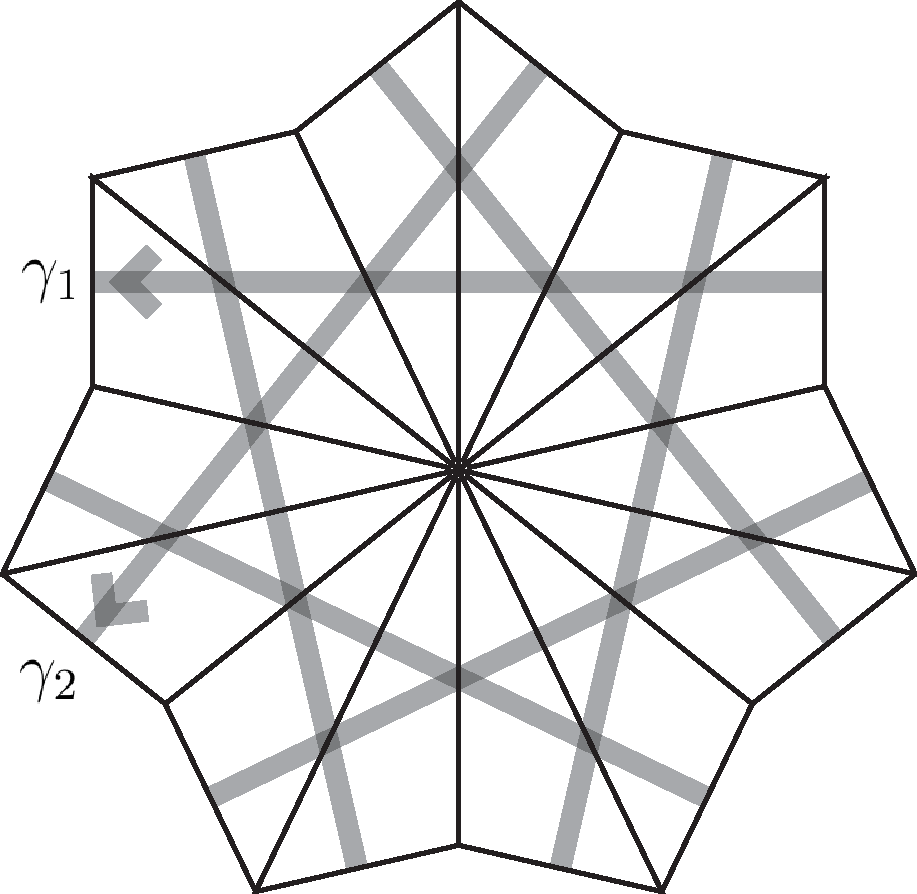
\includegraphics[width=2in]{figures/124_flat.pdf}
\end{minipage}%
\begin{minipage}{0.5\textwidth}
  \centering
  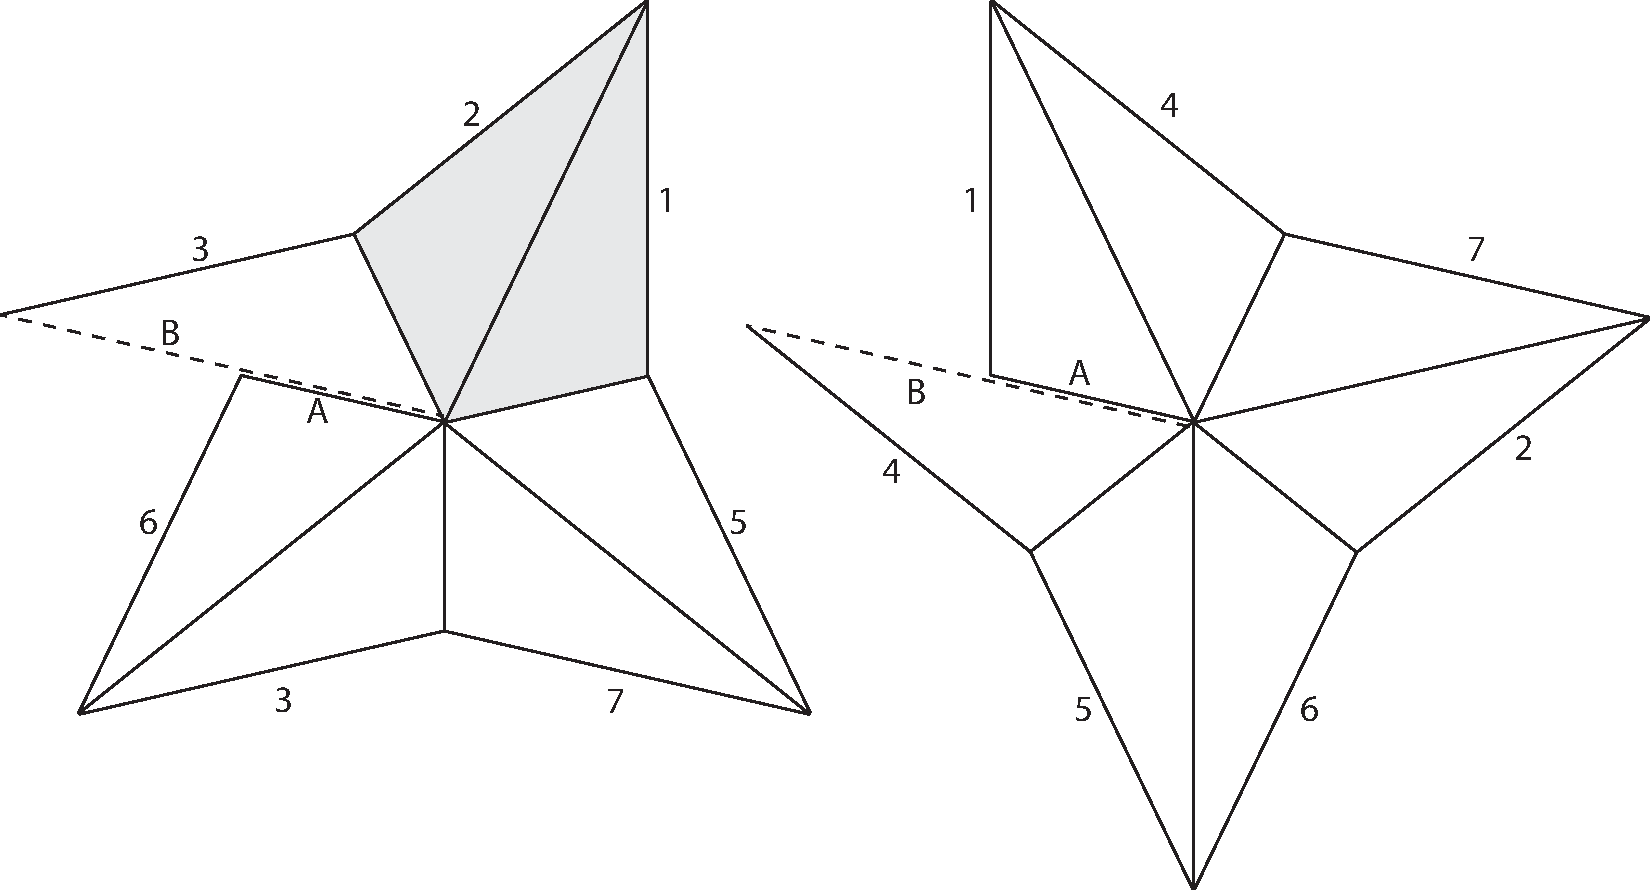
\includegraphics[width=3in]{figures/124_flat_2.pdf}
\end{minipage}
  \caption{Two different flat structures on Klein's quartic.}
  \label{fig:124}
\end{figure}

Along with $\omega_3$ one can compute the period matrix as in Section~\ref{sec:cyclicperiod}.

\subsubsection{Genus three Fermat's quartic}
Fermat's quartic is another genus three non-hyperelliptic curve defined by 8(1,2,5) \cite{dami}. The flat structures are described in Figure~\ref{fig:125_flat} and Figure~\ref{fig:flat_rs2}. The period matrix can be found in Section~\ref{sec:cyclicperiod}. One can write the curve model as $y^8 = x (x-1)^2.$ However, one can also consider a fourfold covering over $\C\P^1$ branched over four points and write it as $y^4 = x (x-1) (x+1).$ See \cite{dami} for details.

\subsubsection{Genus three hyperelliptic curve}
As an example of a hyperelliptic curve, we look into 12(1,5,6). Its quotient under the hyperelliptic involution is $\C\P^1$, where the eight hyperelliptic points are located at the North Pole, South Pole, and at six equidistributed points along the Equator. That is, the curve can be described as $y^2 = x(x^6 -1).$ Figure~\ref{fig:156} describes two different flat structures, one order-4 zero (left), and two order-2 zeros (right).

\begin{figure}[htbp]
\centering
\begin{minipage}{0.5\textwidth}
  \centering
  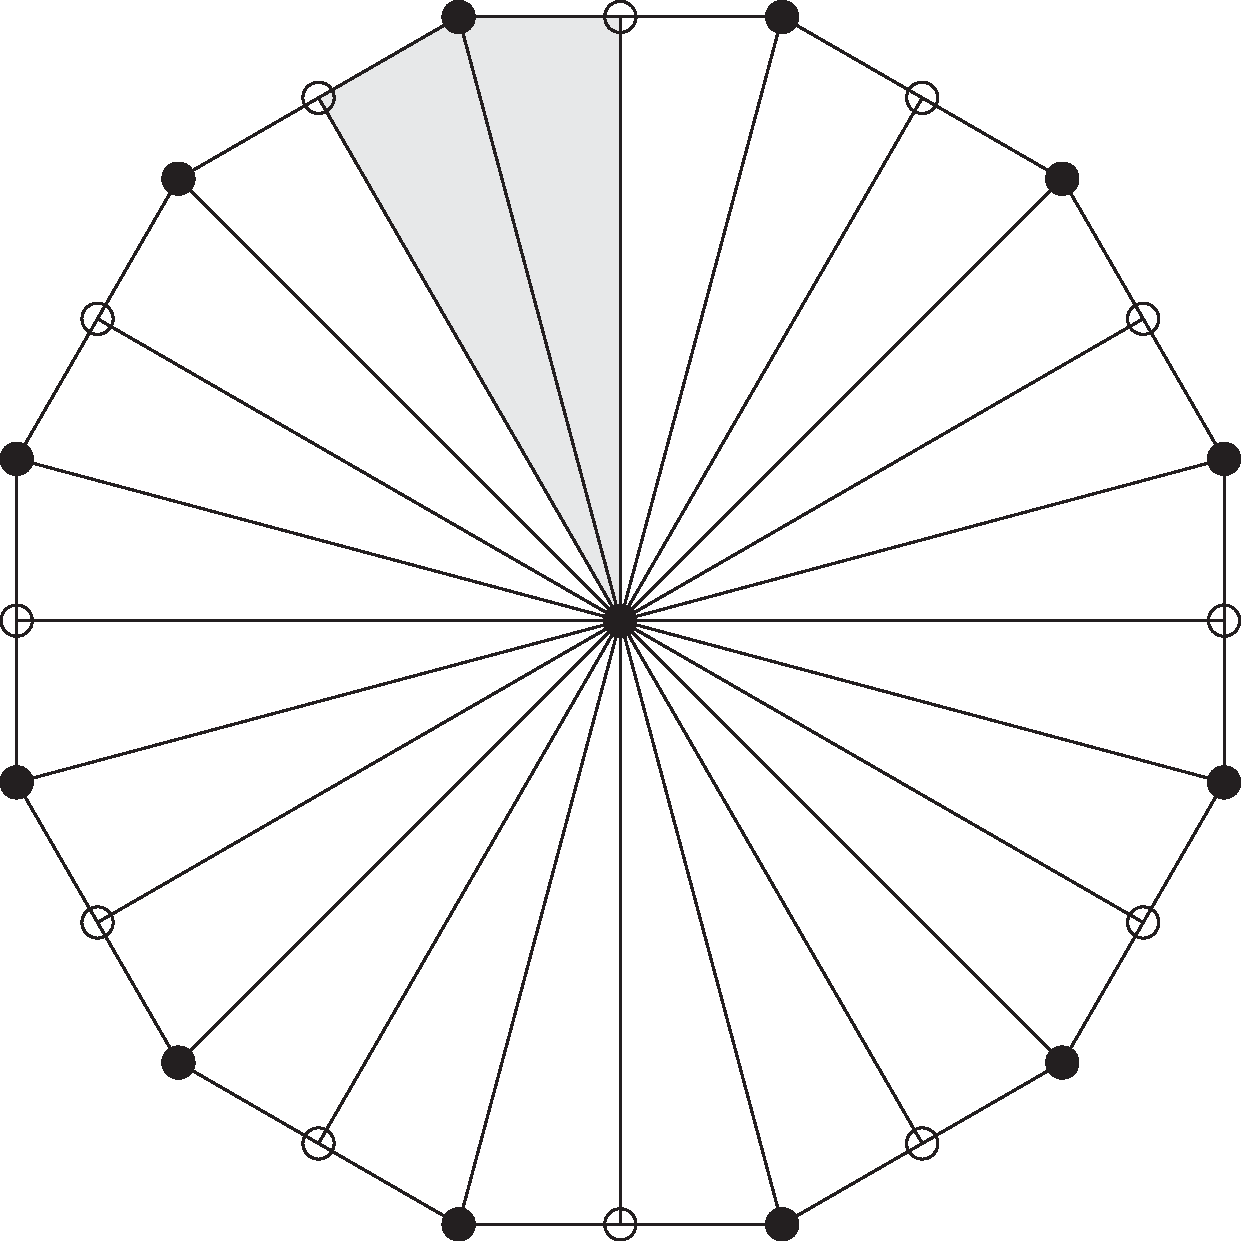
\includegraphics[width=2in]{figures/156_flat.pdf}
\end{minipage}%
\begin{minipage}{0.5\textwidth}
  \centering
  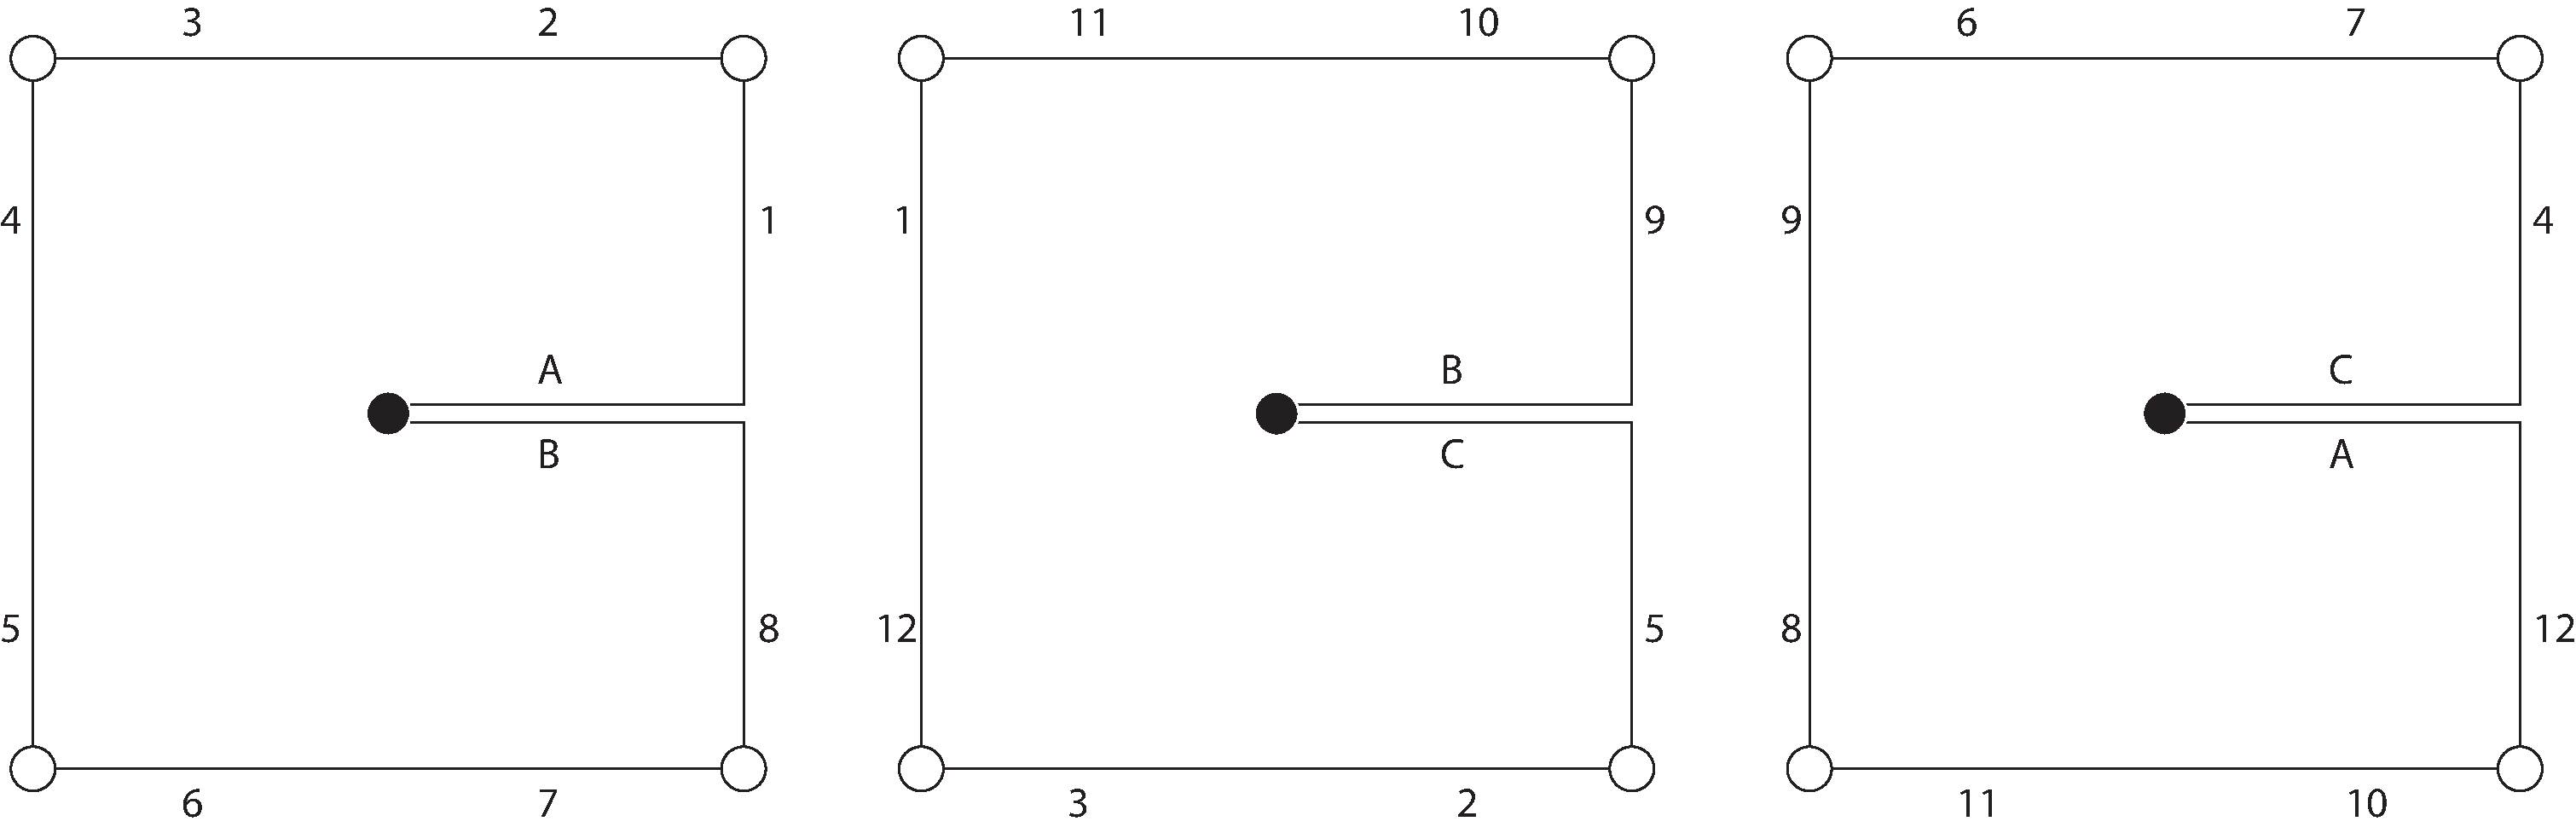
\includegraphics[width=3in]{figures/156_flat_2.pdf}
\end{minipage}
  \caption{Two different flat structures on 12(1,5,6).}
  \label{fig:156}
\end{figure}

\subsubsection{Genus four Bring's curve}
Bring's curve is a genus four non-hyperelliptic curve denoted by 5(1,2,4,3). In \cite{matti}, this curve is presented as $y^5 = x^2(x+1)(x-1)^4$ by choosing $p_i = -1, 0, 1, \infty.$ Figure~\ref{fig:1243} represents two different flat structures $(\omega_1) = \widetilde{p_2} + 3 \widetilde{p_3} + 2 \widetilde{p_4}$ (reprinted from \cite{matti}) and $(\omega_2) = \widetilde{p_1} + 3 \widetilde{p_2} + 2 \widetilde{p_3}.$

\begin{figure}[htbp] %  figure placement: here, top, bottom, or page
\centering
\begin{minipage}{0.5\textwidth}
  \centering
  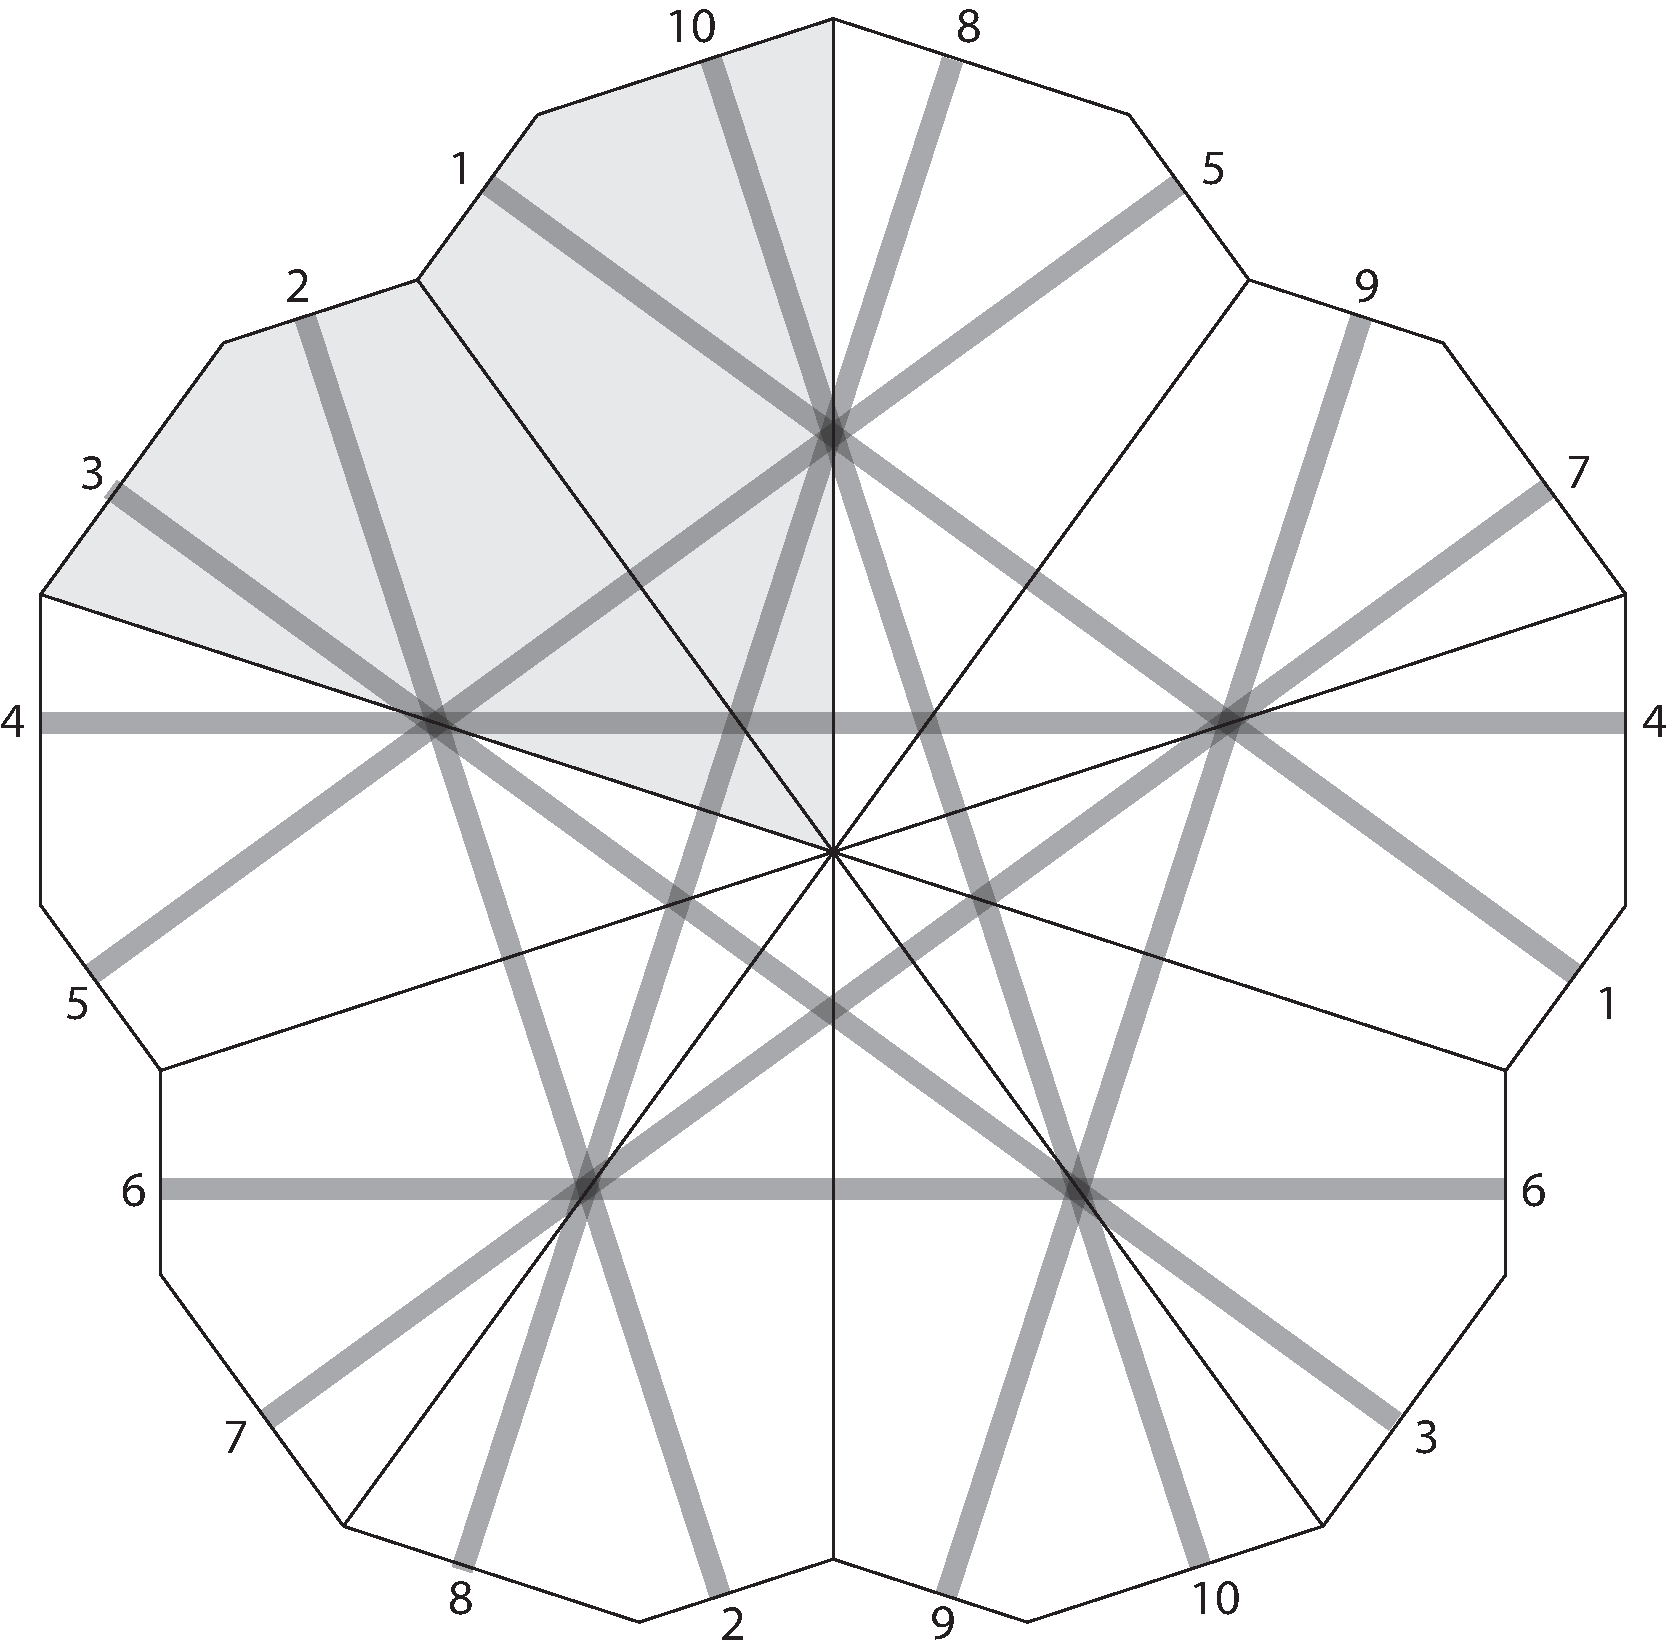
\includegraphics[width=2in]{figures/1243_flat.pdf}
\end{minipage}%
\begin{minipage}{0.5\textwidth}
  \centering
  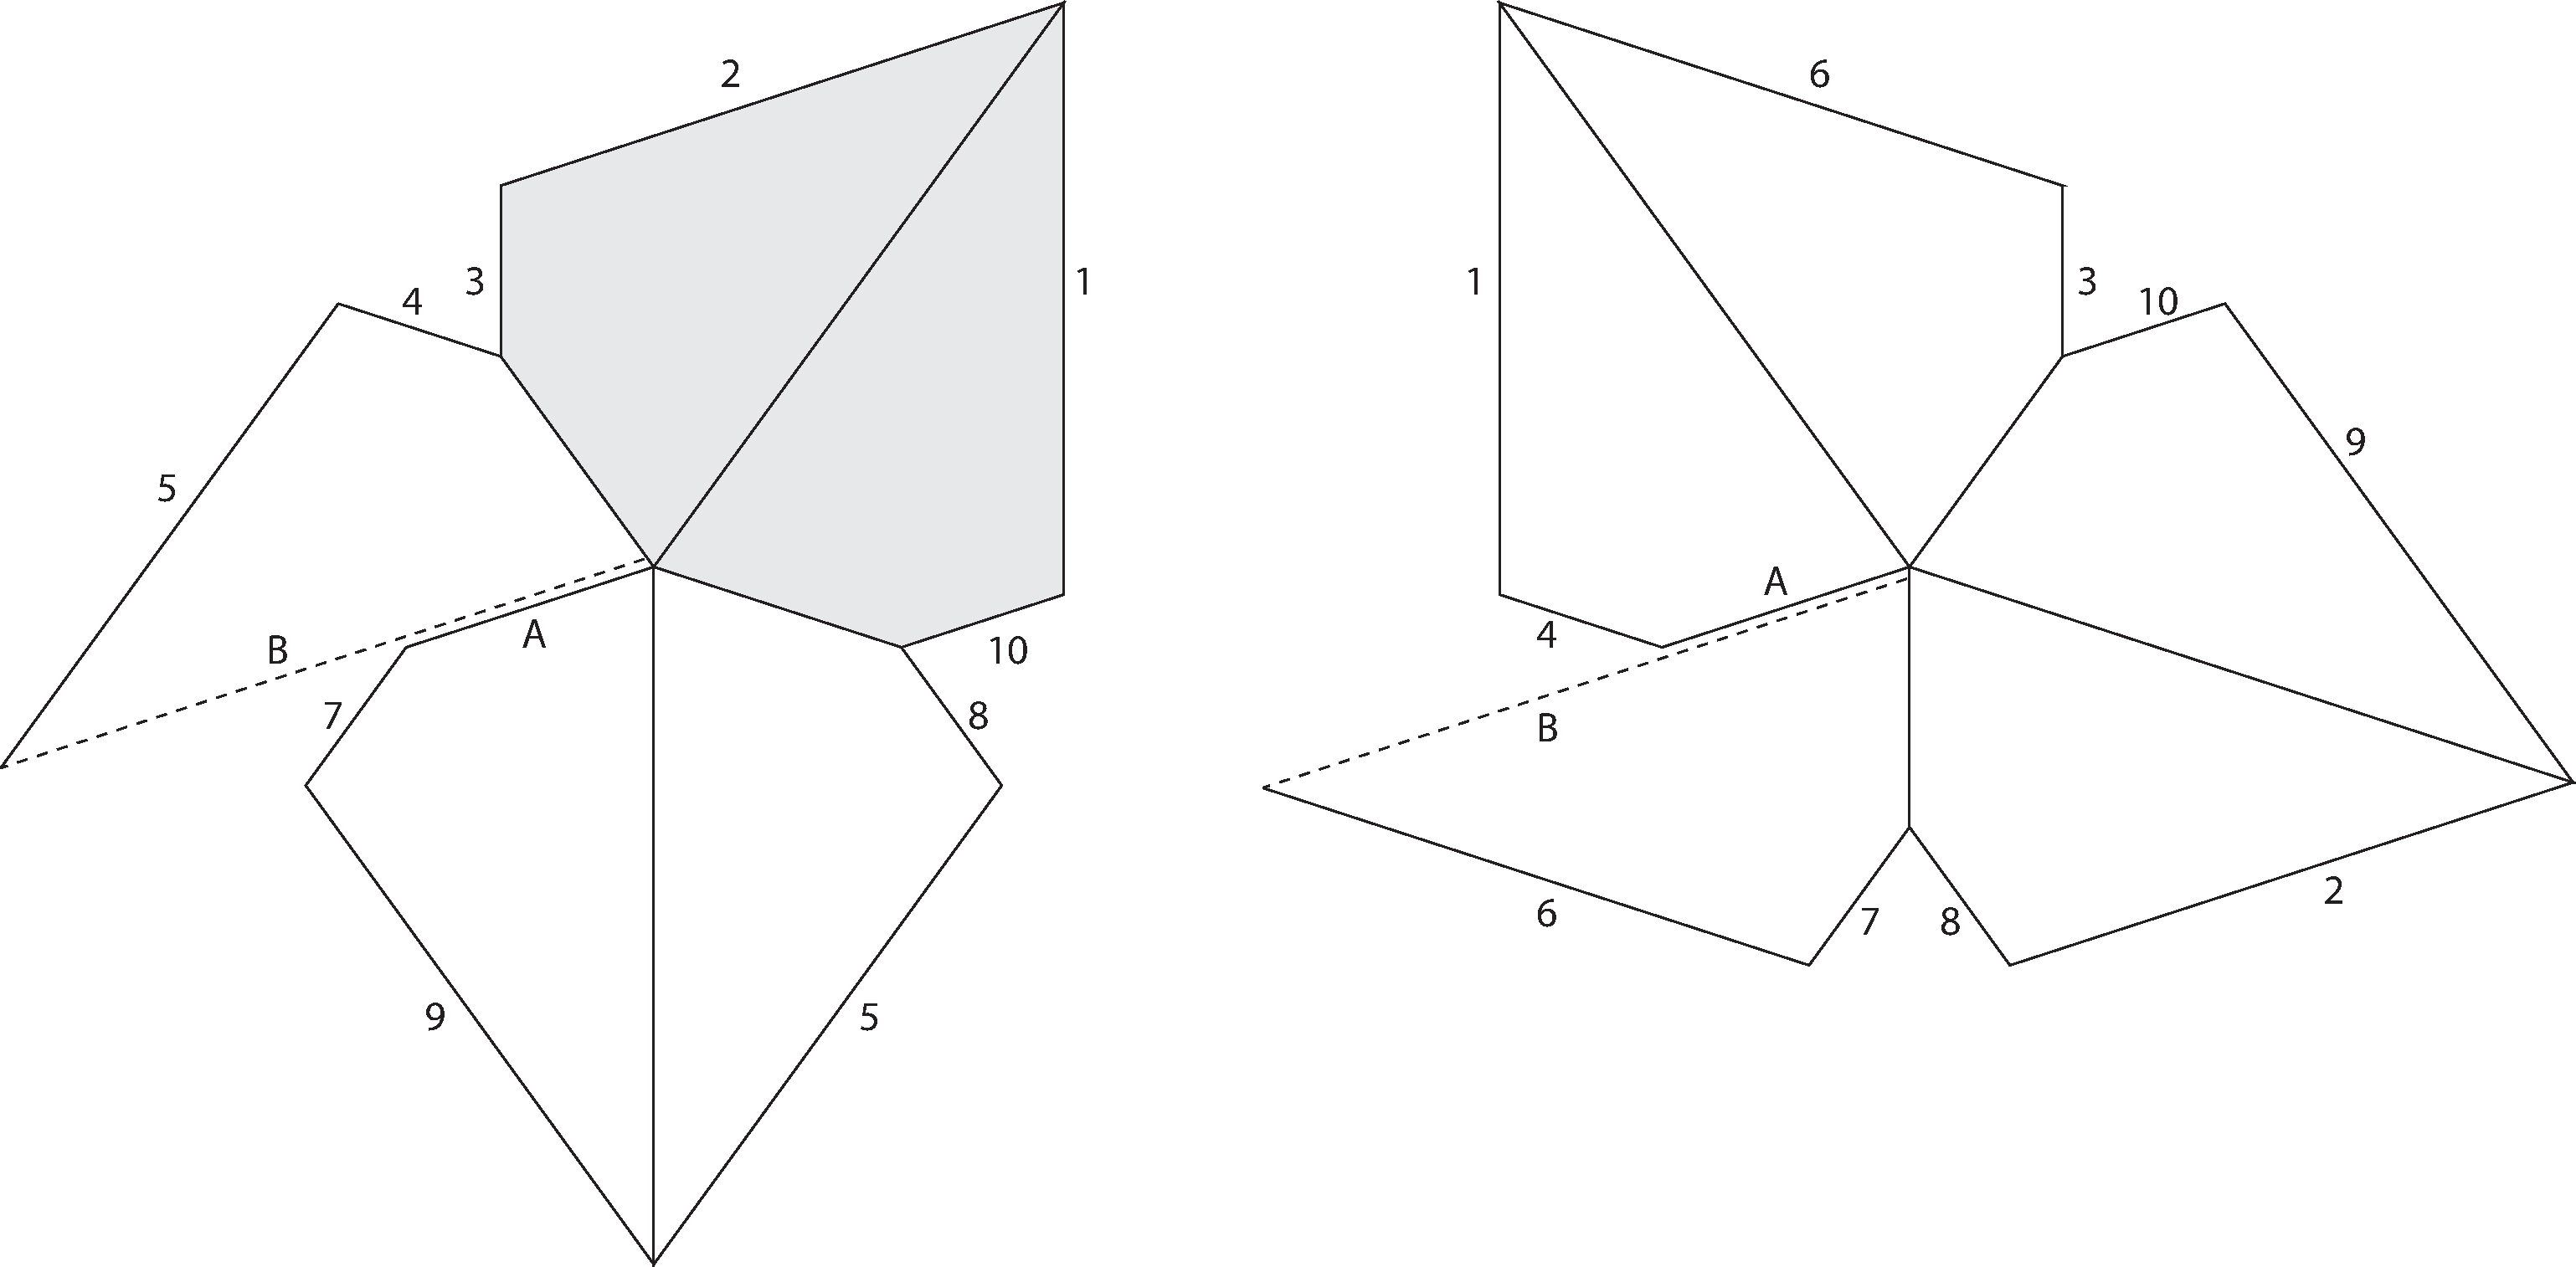
\includegraphics[width=3in]{figures/1243_flat_2.pdf}
\end{minipage}
  \caption{Two different flat structures on Bring's curve.}
  \label{fig:1243}
\end{figure}

\subsubsection{Schoen's I-WP minimal surface}
Lastly, I-WP is another genus four non-hyperelliptic curve defined by 12(1,4,7). This covering presentation is due to Lee \cite{dthesis}, where it is shown that the underlying curve of Schoen's I-WP surface is equipped with cone metrics that are compatible with the twelvefold cyclic cover over $\C\P^1.$ Figure~\ref{fig:147} represents a holomorphic 1-form with one order-6 zero and a 1-form with six simple zeros.

\begin{figure}[htbp] 
\centering
\begin{minipage}{0.5\textwidth}
  \centering
  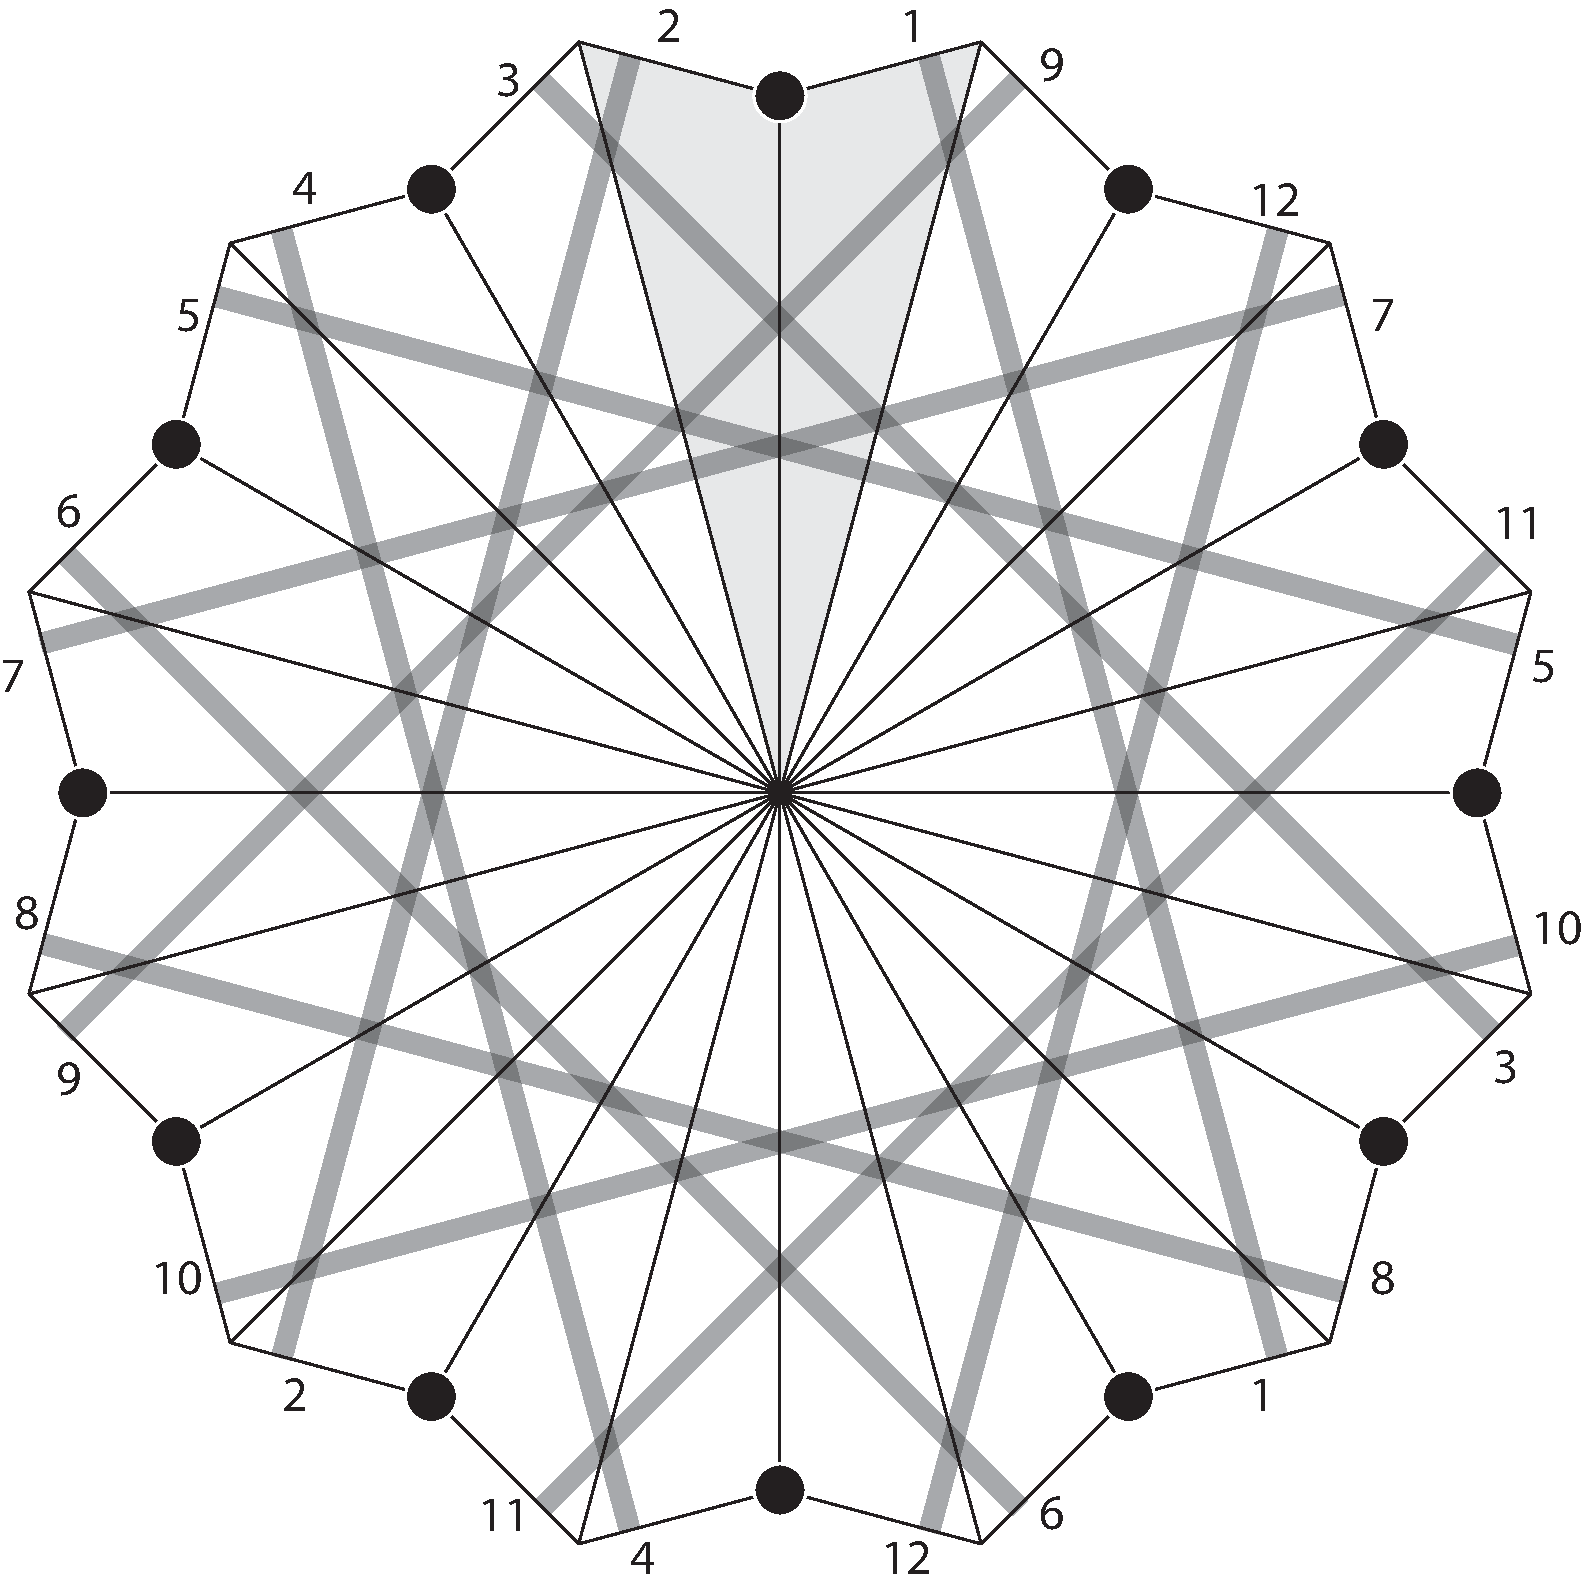
\includegraphics[width=2in]{figures/147_flat.pdf}
\end{minipage}%
\begin{minipage}{0.5\textwidth}
  \centering
  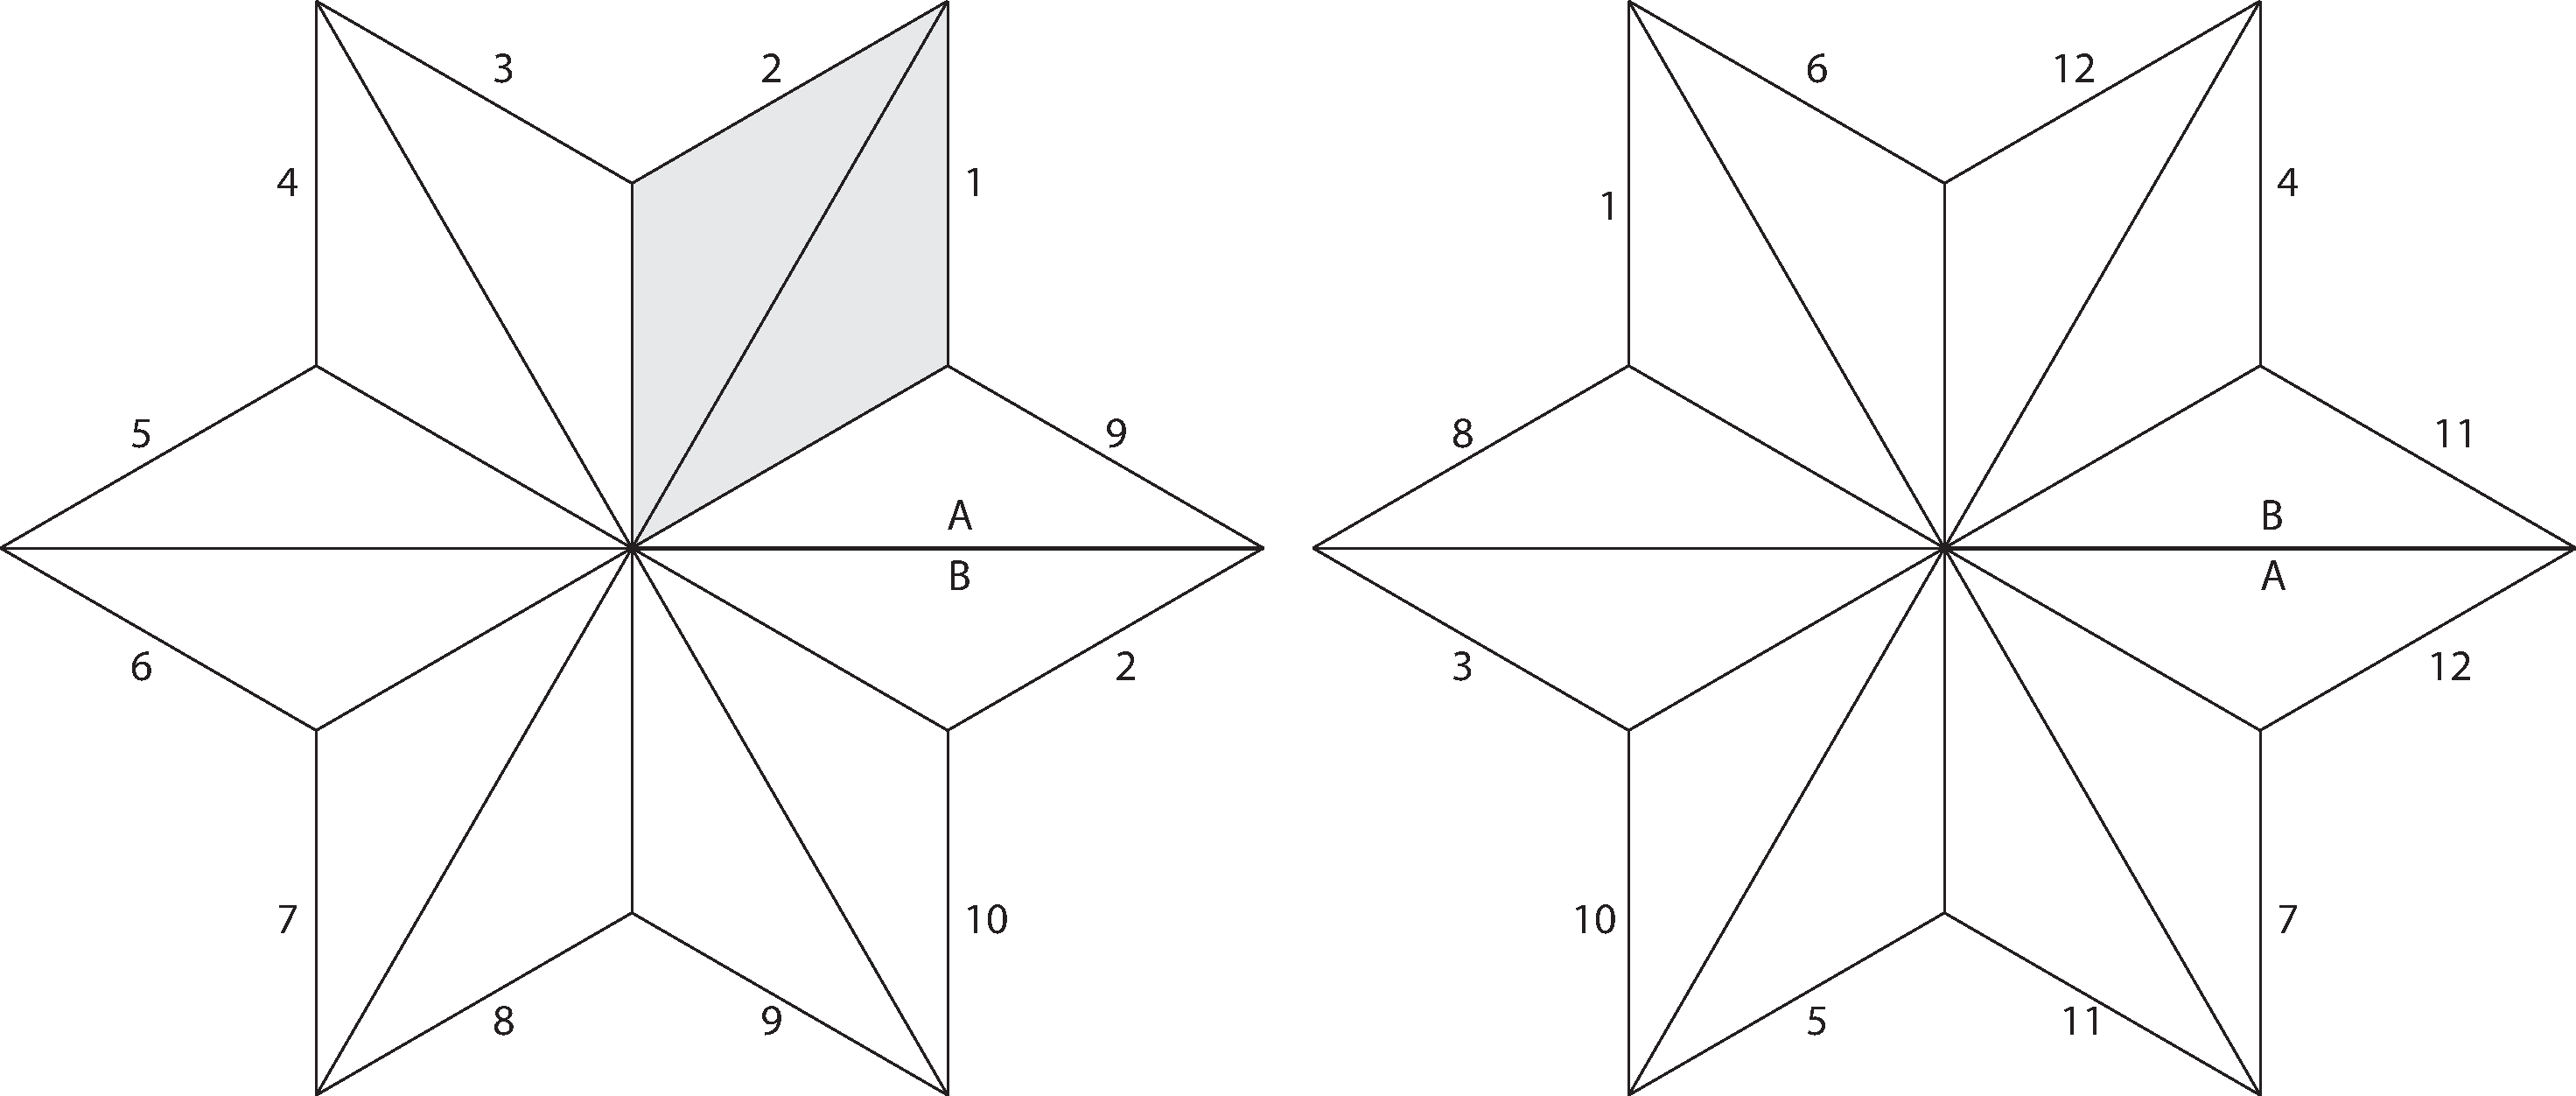
\includegraphics[width=3in]{figures/147_flat_2.pdf}
\end{minipage}
  \caption{Two different flat structures on Schoen's I-WP.}
  \label{fig:147}
\end{figure}

\subsection{Questions and Answers on Abelian Varieties with Multiple Principal Polarizations}
\label{sec:questions}


We speak here of polarizations up to auto-equivalence and ask natural questions on Jacobians with multiple principal polarizations, answering all but one of the questions using methods developed in our paper.

We fix some notation. We call $\Aut(A, a_i)$ a symplectic automorphism group of $A$, as the automorphisms respect the principal polarization $a_i$, which is a symplectic form on $A$. Let $\theta_C$ be the canonical principal polarization of $\Jac(C)$ with respect to $C$.

\begin{question} $\Aut(\Jac(C), \theta_C)$ will have the highest order of all symplectic automorphism groups of $\Jac(C)$. \end{question}

\begin{answer} This is proven false by example $12(1,5,6)$, where $|\Aut(\Jac(12(1, 5, 6)), \theta_{12(1, 5, 6)})| = 24$, but $|\Aut(\Jac(12(1, 5, 6)), a_i)| = 32$ is achieved. It is more dramatically proven false by Schoen's I-WP Surface, where $|\Aut(\Jac(\text{I-WP}), \theta_{\text{I-WP}})| = 288$, but $|\Aut(\Jac(\text{I-WP}), a_i)|$ achieves $576$ and $864$. \end{answer}

\begin{question} Principal polarizations $p_1$ and $p_2$ are auto-equivalent if and only if they are analytically equivalent. In other words, $$\Aut(X, p_1) \simeq \Aut(X, p_2) \Leftrightarrow p_1 = p_2.$$ \end{question}

\begin{answer} The direction ($\Leftarrow$) is true because $\mc{L}$ and $\mc{M}$ are analytically equivalent if and only if $c_1(\mc{L}) = c_1(\mc{M})$ by [\cite{bl} 2.5.3]. The other direction ($\Rightarrow$) is false.  This is proven false by applying our method to the the following two \textit{non-isomorphic} curves with the same \textit{unpolarized} Jacobian from Theorem 1 of \cite{howe1}:
\vspace{-2pt}
$$X: 3y^2 = (2x^2- 2)(16x^4 + 28x^2 + 1)$$ 
\vspace{-15pt}
$$X': -y^2 = (2x^2 + 2)(16x^4 + 12x^2 + 1)$$ 

\noindent which both have $\Aut(\Jac(X), \theta_X)\simeq C_2 \times C_2 \simeq \Aut(\Jac(X'), \theta_{X'})$. \end{answer}

The counterexample to the above question arises by giving an example of a pair non-isomorphic curves $X \nsimeq X'$ with the following two properties: $$\Jac(X) \simeq \Jac(X') \text{  and  }  \Aut(\Jac(X), \theta_X) \simeq \Aut(\Jac(X'), \theta_{X'}).$$ It is natural to ask if this phenomena occurs for \textit{all} pairs of curves with isomorphic unpolarized Jacobians, i.e., if the first property implies the second.

\begin{question} Let $C$ and $C'$ be any curves such that $\Jac(C) \simeq \Jac(C')$ as complex varieties, then $$\Aut(\Jac(C), \theta_C) \simeq \Aut(\Jac(C'), \theta_{C'}).$$  \end{question} 

We checked this question on the family of hyperelliptic cases of genus 2 from \cite{howe1} Theorem 1, where it is true. However, there is no reason to expect this to be true in general. Yet, we cannot disprove it easily. 



\begin{thebibliography}{20}

\bibitem{bl} 
C. Birkenhake, H. Lange, 
\textit{Complex Abelian Varieties},
Springer, 2004.

\bibitem{rigor}
E. Costa, N. Mascot, J. Sijsling, J. Voight
\textit{Rigorous Computation of the Endomorphism Ring of a Jacobian}
Math. Comp. 88 (2019), 1303-1339

\bibitem{numerical}
N. Bruin, J. Sijsling, A. Zotine,
\textit{Numerical Computation of Endomorphism Rings of Jacobians},
\texttt{https://arxiv.org/pdf/1807.02605.pdf}, preprint.

\bibitem{smith}
B. Smith
\textit{Explicit Endomorphisms and Correspondence, PhD Thesis 2005}

\bibitem{elkies}
N. Elkies,
\textit{The automorphism group of the modular curve $X_0(63)$},
Composito Mathematica,
Vol. 74, 1986, pp.127--152.

\begin{comment}
\bibitem{fk}
H. Farkas, I. Kra,
\textit{Riemann Surfaces},
Springer-Verlag, New York, 1992.
\end{comment} 

\bibitem{howe1}
E. Howe,
\textit{Constructing Distinct Curves with Isomorphic Jacobians},
Journal of Number Theory,
Vol. 56, Issue 2, 1996, pp.381--390.

\bibitem{howe2} 
E. Howe,
\textit{Infinite families of pairs of curves over $\Q$ with Isomorphic Jacobians},
Journal of the London Mathematical Society,
Vol. 72, Issue 2, 2005, pp.327--350.

\bibitem{iko}
T. Ibukiyama, T. Katsura, F. Oort,
\textit{Supersingular curves of genus two and class numbers},
Composito Mathematica,
Vol. 57, No. 2, 1986, pp.127--152.

\bibitem{kw}
H. Karcher, M. Weber,
\textit{On Klein's Riemann Surface},
The Eightfold Way, MSRI Publications, 
Vol. 35, 1998, pp.9--49.

\bibitem{km}
M. A. Kenku, F. Momose,
\textit{Automorphism Groups of the modular curves $X_0(N)$},
Composito Mathematica,
Vol. 65, No. 1, 1988, pp.51--80.

\bibitem{several} 
H. Lange,
\textit{Abelian Varieties with Several Principal Polarizations},
Duke Mathematical Journal,
Vol. 55, Number 3, 1987, pp.617--628.

\bibitem{newlange}
H. Lange
\textit{Principal Polarizations on Products of Elliptic Curves}
Contemporary Mathematics, Vol. 397, 2006, pp.153--162

\bibitem{dami} 
D. Lee,
\textit{On a triply periodic polyhedral surface whose vertices are Weierstrass points},
Arnold Mathematical Journal, 
Vol. 3, Issue 3, 2017, pp.319--331.

\bibitem{dthesis} 
D. Lee, 
\textit{Geometric realizations of cyclically branched coverings over punctured spheres}, 
Ph.D thesis, 2018.
 
 
\bibitem{hyp}
R. Lercier, C. Ritzenthaler, J. Sijsling,
\textit{Fast computation of isomorphisms of hyperelliptic curves and explicit Galois descent},
Proceedings of the Tenth Algorithmic Number Theory Symposium, 2013, pp. 463–-486.

\bibitem{n}
N. Mascot,
\textit{Computing modular Galois representations},
Rendiconti del Circolo Matematico di Palermo,
Vol. 62, Issue. 3, 2013, pp.451--476.

\bibitem{nn} 
M. S. Narasimhan, M. V. Nori,
\textit{Polarisations on an abelian variety},
Proceedings of the Indian Academy of Sciences,
Vol. 90, 1951, pp.125--128.


\bibitem{matti} 
M. Weber,
\textit{Kepler's small stellated dodecahedron as a Riemann surface},
Pacific Journal of Mathematics, 
Vol. 220, 2005, pp.167--182.

\bibitem{Torelli}
K. Lauter, J.-P., Serre, 
\textit{Geometric Methods for Improving the Upper Bounds on the Number of Rational Points on Algebraic Curves over Finite Fields}, 
Journal of Algebraic Geometry,
Vol. 10, 2001.

\bibitem{oe}
A. Weil,
\textit{Oeuvres Scientifiques},
Springer,
Vol. 2, 1983.

\bibitem{finn}
H. Martens,
\textit{A New Proof of Torelli's Theorem},
Annals of Mathematics,
Second Series, Vol. 78, No. 1, 1963, pp.107--111.


\end{thebibliography}
\end{document}
